\documentclass{ximera}

\begin{document}
	\author{Stitz-Zeager}
	\xmtitle{TITLE}


\label{ExercisesforAppDerivatives}
In Exercises \ref{diffquotexerfirsta} - \ref{diffquotexerlasta}, find the limit of the following difference quotients.

\begin{multicols}{2}

\begin{itemize}

\item  $\ds{\lim_{h \rightarrow 0} \dfrac{f(2+h) - f(2)}{h}}$

\item  $\ds{\lim_{h \rightarrow 0} \dfrac{f(x+h) - f(x)}{h}}$

\end{itemize}

\end{multicols}


\begin{multicols}{2}

\begin{enumerate}


\item $f(x) = 2x - 5$ \label{diffquotexerfirsta}
\item $f(x) = -3x + 5$

\setcounter{HW}{\value{enumi}}
\end{enumerate}
\end{multicols}

\begin{multicols}{2}
\begin{enumerate}
\setcounter{enumi}{\value{HW}}

\item $f(x) = 6$
\item $f(x) = 3x^2 - x$

\setcounter{HW}{\value{enumi}}
\end{enumerate}
\end{multicols}

\begin{multicols}{2}
\begin{enumerate}
\setcounter{enumi}{\value{HW}}

\item $f(x) = -x^2 + 2x - 1$
\item\label{diffquotexerlasta}  $f(x) = 4x^2$ 

\setcounter{HW}{\value{enumi}}
\end{enumerate}
\end{multicols}


In Exercises \ref{tangentlinepolyfirst} - \ref{tangentlinepolylast}, find:


\begin{itemize}

\item  $f'(2)  = \ds{\lim_{h \rightarrow 0} \dfrac{f(2+h) - f(2)}{h}}$

\item  The equation of the tangent line at $(2, f(2))$.  Check your answer graphically.

\item  $f'(x) = \ds{\lim_{h \rightarrow 0} \dfrac{f(x+h) - f(x)}{h}}$

\item  The equation of the tangent line at $(0,f(0))$.  Check your answer graphically.
 
\end{itemize}



\begin{multicols}{2}
\begin{enumerate}
\setcounter{enumi}{\value{HW}}

\item\label{tangentlinepolyfirst}  $f(x) = x-x^2$ 
\item\label{tangentlinepolylast} $f(x) = x^{3} + 1$

\setcounter{HW}{\value{enumi}}
\end{enumerate}
\end{multicols}




\begin{enumerate}
\setcounter{enumi}{\value{HW}}

\item  Find $f'(x) = \ds{\lim_{h \rightarrow 0} \dfrac{f(x+h) - f(x)}{h}}$  for $f(x) = mx + b\;$ where $m \neq 0$

\item\label{quadraticderivativeformulaexercise} \begin{enumerate}  \item Find $f'(x) = \ds{\lim_{h \rightarrow 0} \dfrac{f(x+h) - f(x)}{h}}$   for  $f(x) = ax^{2} + bx + c\;$ where $a \neq 0$.

\item  Solve $f'(x) = 0$ for $x$.  Does this look familiar?  Explain.

\end{enumerate}

\setcounter{HW}{\value{enumi}}
\end{enumerate}





In Exercises \ref{diffquotexerfirstb} - \ref{diffquotexerlastb}, find the limit of the following difference quotients:

\begin{multicols}{2}

\begin{itemize}

\item  $\ds{\lim_{\Delta x \rightarrow 0} \dfrac{f(-1+\Delta x) - f(-1)}{\Delta x}}$

\item  $\ds{\lim_{\Delta x \rightarrow 0} \dfrac{f(x+\Delta x) - f(x)}{\Delta x}}$

\end{itemize}

\end{multicols}

\begin{multicols}{2}
\begin{enumerate}
\setcounter{enumi}{\value{HW}}

\item $f(x) = \dfrac{2}{x}$  \label{diffquotexerfirstb}
\item $f(x) = \dfrac{3}{1-x}$

\setcounter{HW}{\value{enumi}}
\end{enumerate}
\end{multicols}

\begin{multicols}{2}
\begin{enumerate}
\setcounter{enumi}{\value{HW}}

\item  $f(x) = \dfrac{1}{x^2}$
\item\label{diffquotexerlastb}  $f(x) = \dfrac{2}{x+5}$

\setcounter{HW}{\value{enumi}}
\end{enumerate}
\end{multicols}

In Exercises \ref{rationaltangentfirst} - \ref{rationaltangentlast}, find the limit of the following:



\begin{itemize}

\item  $f'(-1) = \ds{\lim_{\Delta x \rightarrow 0} \dfrac{f(-1+\Delta x) - f(-1)}{\Delta x}}$

\item The equation of the tangent line at $(-1, f(-1))$.

\item  $f'(x) = \ds{\lim_{\Delta x \rightarrow 0} \dfrac{f(x+\Delta x) - f(x)}{\Delta x}}$

\item  The equation of the tangent line at $(0,f(0))$.

\end{itemize}

\begin{multicols}{2}
\begin{enumerate}

\setcounter{enumi}{\value{HW}}

\item\label{rationaltangentfirst} $f(x) = \dfrac{1}{4x-3}$ 
\item $f(x) = \dfrac{3x}{x+2}$ 

\setcounter{HW}{\value{enumi}}
\end{enumerate}
\end{multicols}

\begin{multicols}{2}
\begin{enumerate}
\setcounter{enumi}{\value{HW}}

\item $f(x) = \dfrac{x}{x - 9}$
\item\label{rationaltangentlast} $f(x) = \dfrac{x^2}{2x+1}$ 

\setcounter{HW}{\value{enumi}}
\end{enumerate}
\end{multicols}

In Exercises \ref{diffquotexerfirstc} - \ref{diffquotexerlastc},  find the limit of the following difference quotients:

\begin{multicols}{2}

\begin{itemize}

\item  $\ds{\lim_{\Delta t \rightarrow 0} \dfrac{g(\Delta t) - g(0)}{\Delta t}}$

\item  $\ds{\lim_{\Delta t \rightarrow 0} \dfrac{g(t+\Delta t) - g(t)}{\Delta t}}$

\end{itemize}

\end{multicols}


\begin{multicols}{2}
\begin{enumerate}
\setcounter{enumi}{\value{HW}}

\item  $g(t) = \sqrt{9-t}$  \label{diffquotexerfirstc}
\item  $g(t) = \sqrt{2t+1}$   \label{diffquotexerlastc}


\setcounter{HW}{\value{enumi}}
\end{enumerate}
\end{multicols}

In Exercises \ref{tangentrootfirst} - \ref{tangentrootlast},  find the following:



\begin{itemize}

\item  $g'(0) = \ds{\lim_{\Delta t \rightarrow 0} \dfrac{g(\Delta t) - g(0)}{\Delta t}}$

\item  The equation of the tangent line at $(0, g(0))$.

\item  $g'(t) =  \ds{\lim_{\Delta t \rightarrow 0} \dfrac{g(t+\Delta t) - g(t)}{\Delta t}}$

\item  The equation of the tangent line at $(1, g(1))$.

\end{itemize}




\begin{multicols}{2}
\begin{enumerate}
\setcounter{enumi}{\value{HW}}

\item\label{tangentrootfirst}  $g(t) = \sqrt{-4t+5}$
\item  \label{tangentrootlast} $g(t) = \sqrt{4-t}$


\setcounter{HW}{\value{enumi}}
\end{enumerate}
\end{multicols}



\begin{enumerate}
\setcounter{enumi}{\value{HW}}

\item  For  $g(t) = t \sqrt{t}$:

\begin{enumerate}

\item  Explain why $g'(0) = \ds{\lim_{\Delta t \rightarrow 0} \dfrac{g(\Delta t) - g(0)}{\Delta t}}$ does not exist.

\item Find the \index{derivative from the right}\index{derivative ! from the right} derivative \textbf{from the right} at $t=0$:  $g_{+}'(0) = \ds{\lim_{\Delta t \rightarrow 0^{+}} \dfrac{g(\Delta t) - g(0)}{\Delta t}}$

\item  Find $y = g_{+}'(0) (x-0) + g(0)$ and interpret.

\item Find  $g'(t) =  \ds{\lim_{\Delta t \rightarrow 0} \dfrac{g(t+\Delta t) - g(t)}{\Delta t}}$.  Assume $t>0$.

\end{enumerate}


\item  \begin{enumerate} \item Find  $g'(t) =  \ds{\lim_{\Delta t \rightarrow 0} \dfrac{g(t+\Delta t) - g(t)}{\Delta t}}$ for  $g(t) = \sqrt{at+b}$, $a \neq 0$. 

\smallskip

\item What restrictions do you place on $t$ so your formula is valid?

\end{enumerate}


\setcounter{HW}{\value{enumi}}
\end{enumerate}


\begin{enumerate}
\setcounter{enumi}{\value{HW}}

\item Let  $f(x) =|x|$.  

\begin{enumerate}

\item  Explain why $f$ is continuous at $x = 0$.

\item\label{cornerex} Show $f'(0)$ does not exist by showing $\ds{\lim_{h \rightarrow 0^{-}} \dfrac{f(h) - f(0)}{h} =-1}$ but  $\ds{\lim_{h \rightarrow 0^{+}} \dfrac{f(h) - f(0)}{h} = 1}$.  

\smallskip
        
\item  Graph $y = f(x)$ near $(0,0)$.  Interpret your answer to number \ref{cornerex} graphically.

\smallskip

\item  Find and simplify  $f'(x) =  \ds{\lim_{h \rightarrow 0} \dfrac{|x+h| - |x|}{h}}$ assuming $x \neq 0$.

\smallskip

\textbf{HINT:}  Consider the two cases $x > 0$ and $x < 0$ \ldots
        
\smallskip

\end{enumerate}


\item Let  $g(t) = \sqrt[3]{t}$.  

\begin{enumerate}

\item Explain why $g$ is continuous at $t = 0$.

\item\label{verticaltangentex} Show $g'(0)$ does not exist by showing $\ds{\lim_{\Delta t \rightarrow 0} \dfrac{g(\Delta t) - g(0)}{\Delta t} = \infty}$.  

\smallskip
        
\item  Graph $y = g(t)$ near $(0,0)$.  Interpret your answer to number \ref{verticaltangentex} graphically.

\smallskip

\item  Find and simplify  $g'(t) =  \ds{\lim_{\Delta t \rightarrow 0} \dfrac{g(t+\Delta t) - g(t)}{\Delta t}}$ assuming $t \neq 0$.

\smallskip

\textbf{HINT:}  $(a-b)\left(a^2+ab+b^2\right) = a^3 - b^3$ 
        
\smallskip

\end{enumerate}

\item Let  $h(x) = x^{\frac{2}{3}}$.  

\begin{enumerate}

\item Explain why $h$ is continuous at $x = 0$.

\item\label{cuspex} Show $h'(0)$ does not exist by showing $\ds{\lim_{\Delta x \rightarrow 0^{-}} \dfrac{h(\Delta x) - h(0)}{\Delta x} = -\infty}$ and $\ds{\lim_{\Delta x \rightarrow 0^{+}} \dfrac{h(\Delta x) - h(0)}{\Delta x} = \infty}$

\smallskip
        
\item  Graph $y = h(x)$ near $(0,0)$.  Interpret your answer to number \ref{cuspex} graphically.

\smallskip

\item  Find and simplify  $h'(x) =  \ds{\lim_{\Delta x \rightarrow 0} \dfrac{h(x+\Delta x) - h(x)}{\Delta x}}$ assuming $x \neq 0$.

\smallskip

\textbf{HINT:}  $(a-b)\left(a^2+ab+b^2\right) = a^3 - b^3$ and $a^2 - b^2 = (a+b)(a-b)$.
        
\smallskip

\end{enumerate}

\item  Recall from Exercise \ref{JasonHammerExercise1} in Section \ref{QuadraticFunctions} that Carl's friend Jason participates in the Highland Games. In one event, the hammer throw, the height $h(t)$ in feet of the hammer above the ground $t$ seconds after Jason lets it go is modeled by the function $h(t) = -16t^2 +  22.08t + 6$. 

\begin{enumerate}

\item  Find and simplify a formula for the velocity of the hammer, $v(t) = h'(t) = \ds{\lim_{\Delta t \rightarrow 0} \dfrac{h(t + \Delta t) - h(t)}{\Delta t}}$.

\item  Find and interpret $v(0)$.

\item  Solve $v(t) = 0$ and interpret.

\item  Find the velocity of the hammer when it hits the ground, rounded to three decimal places.

\end{enumerate}

\item  In Exercise \ref{fueleconomyexercise}  in Section \ref{QuadraticFunctions}, the average fuel economy $F(t)$ in miles per gallon (mpg) for passenger cars in the US $t$ years after 1980 is modeled by  $F(t) = -0.0076t^2+0.45t + 16$, $0 \leq t \leq 28$. 

\begin{enumerate}

\item  Find and simplify a formula for  $F'(t) = \ds{\lim_{h \rightarrow 0} \dfrac{F(t + h) - F(t)}{h}}$.

\item\label{fueleconomytrendexercise}  Find and interpret $F'(0)$, $F'(5)$ and $F'(10)$.

\item  Interpret the trend you observe in your answers to part \ref{fueleconomytrendexercise}.

\end{enumerate}

\item\label{MarginalCostDerivativeExercise} Let us return to Example \ref{marginalsetupex} where  $C(x) = .03x^{3} - 4.5x^{2} + 225x + 250$ denotes the cost, in dollars,  of producing $x$ PortaBoy game systems.

\begin{enumerate}

\item  Find and interpret $C'(75) = \ds{\lim_{h \rightarrow 0} \dfrac{C(75+h) - C(75)}{h}}$.

\item  Recall in Exercise \ref{AverageCostMarginalCostExercise} in Section \ref{FunctionArithmetic}, we found the marginal cost, $MC(75) = 58.53$,   which means it will cost an additional $\$ 58.53$ to produce the $76$th item.  Compare $C'(75)$ and $MC(75)$. 

\end{enumerate}

\setcounter{HW}{\value{enumi}}
\end{enumerate}

\newpage


In Exercises \ref{MatchFcnDerivative1first} - \ref{MatchFcnDerivative1last}, match the graph of the function with a plausible graph of its derivative.

\begin{center}

\begin{multicols}{2}

\begin{enumerate}
\setcounter{enumi}{\value{HW}}

\item \label{MatchFcnDerivative1first}$y = f(x)$:

\setcounter{HW}{\value{enumi}}
\end{enumerate}

Graph A:

\end{multicols}


\begin{multicols}{2}

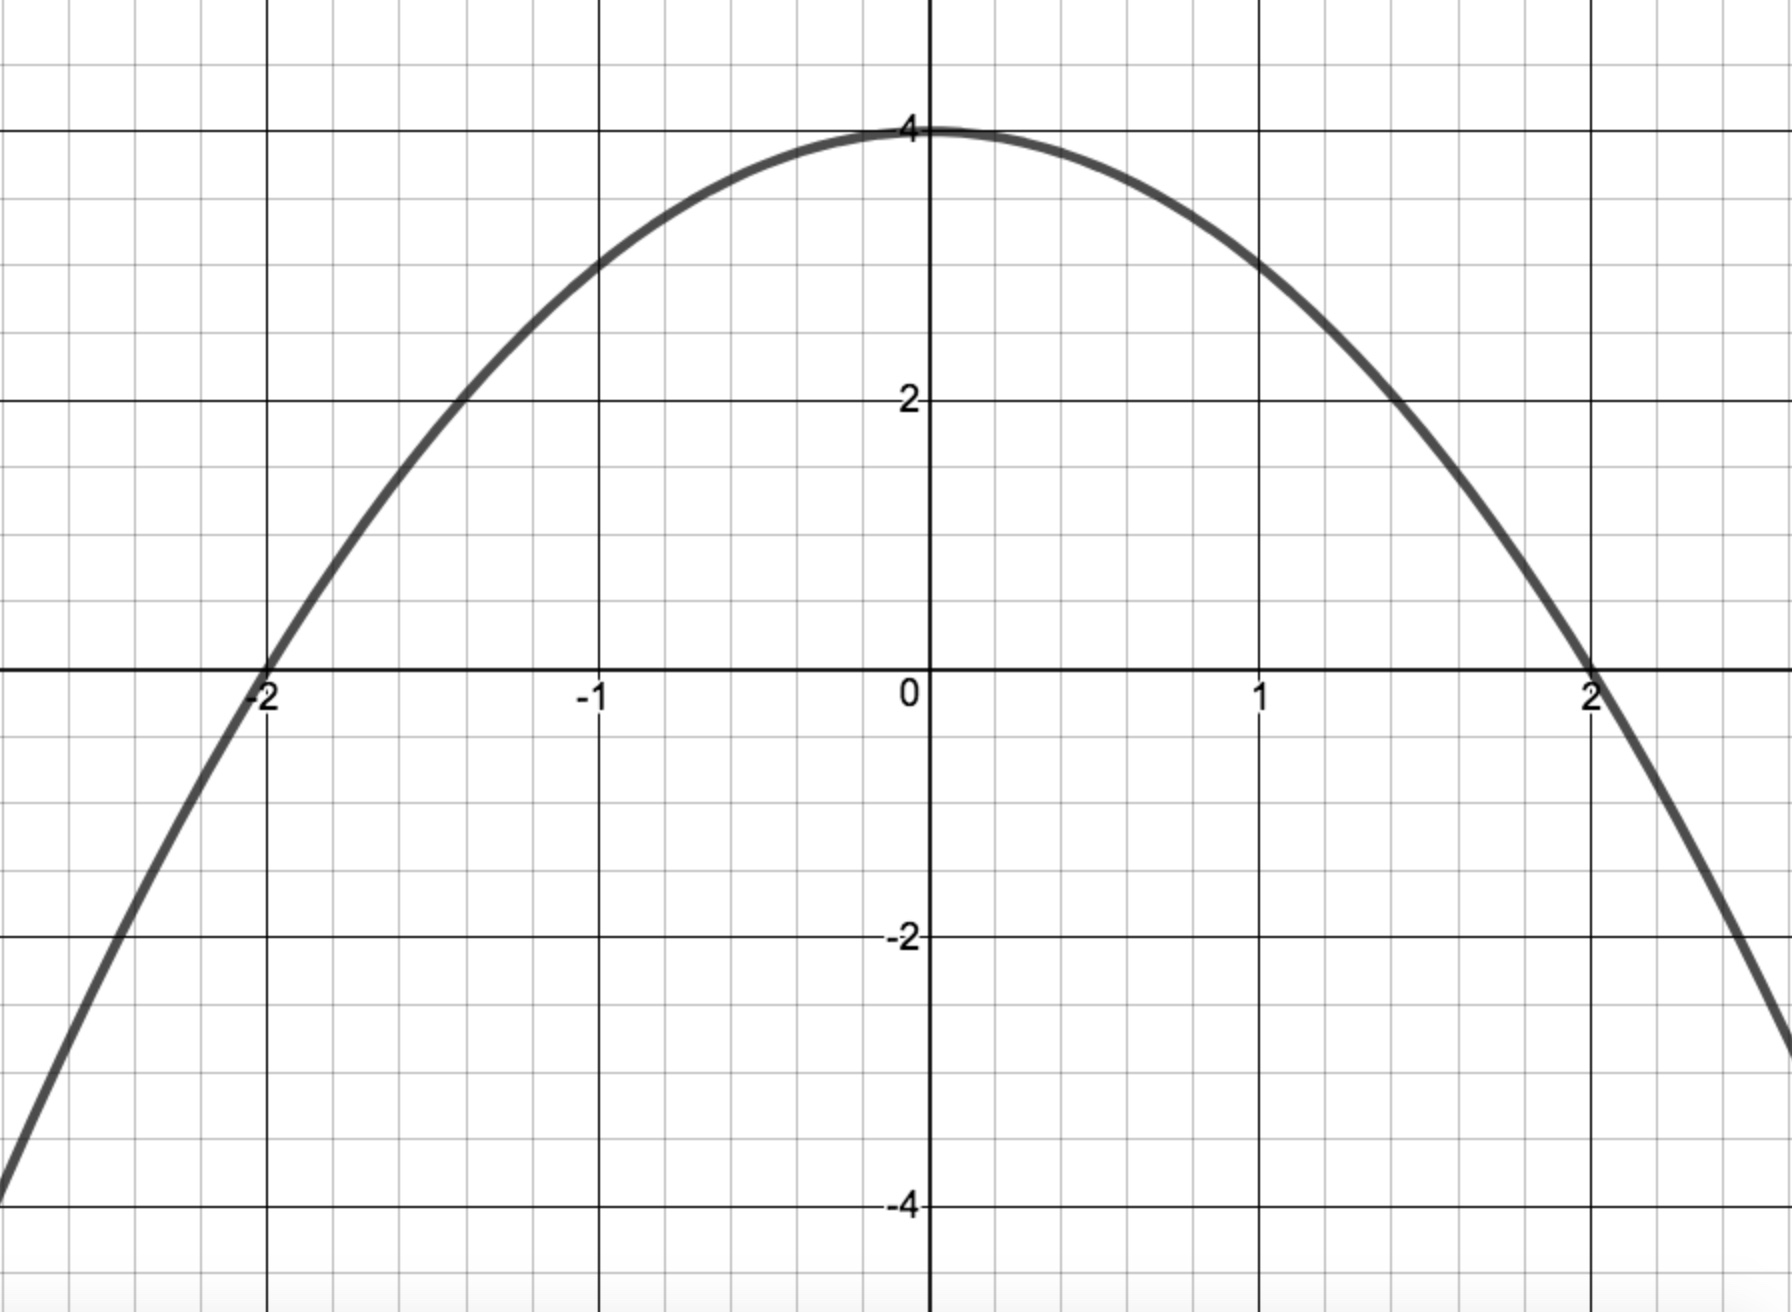
\includegraphics[width=2.75in]{./IntroductiontoDerivativesGraphics/MatchFunc01.jpeg}

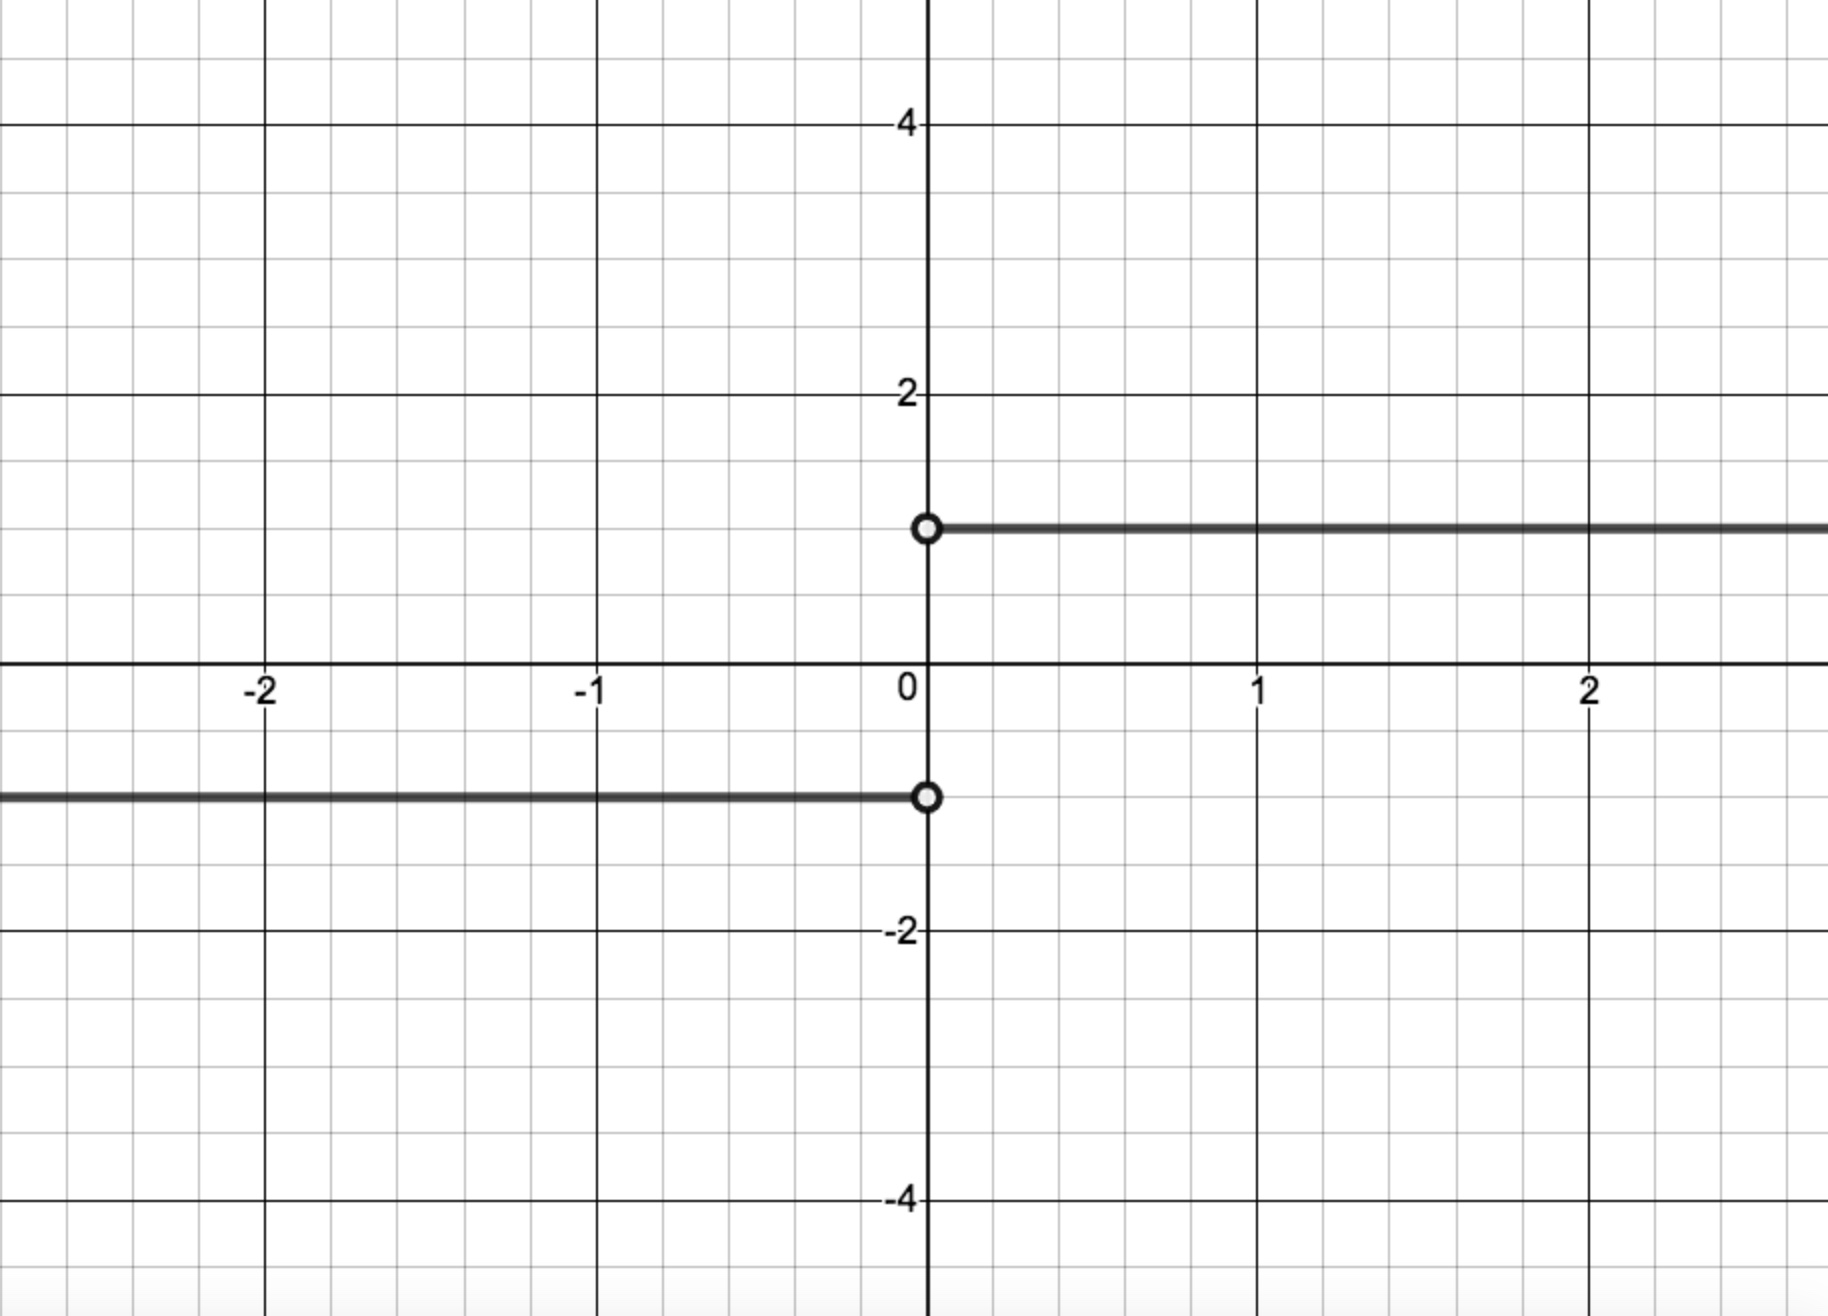
\includegraphics[width=2.75in]{./IntroductiontoDerivativesGraphics/MatchDeriv03.jpeg}

\end{multicols}



\begin{multicols}{2}

\begin{enumerate}
\setcounter{enumi}{\value{HW}}

\item $y = g(x)$:

\setcounter{HW}{\value{enumi}}
\end{enumerate}

Graph B:

\end{multicols}

\begin{multicols}{2}

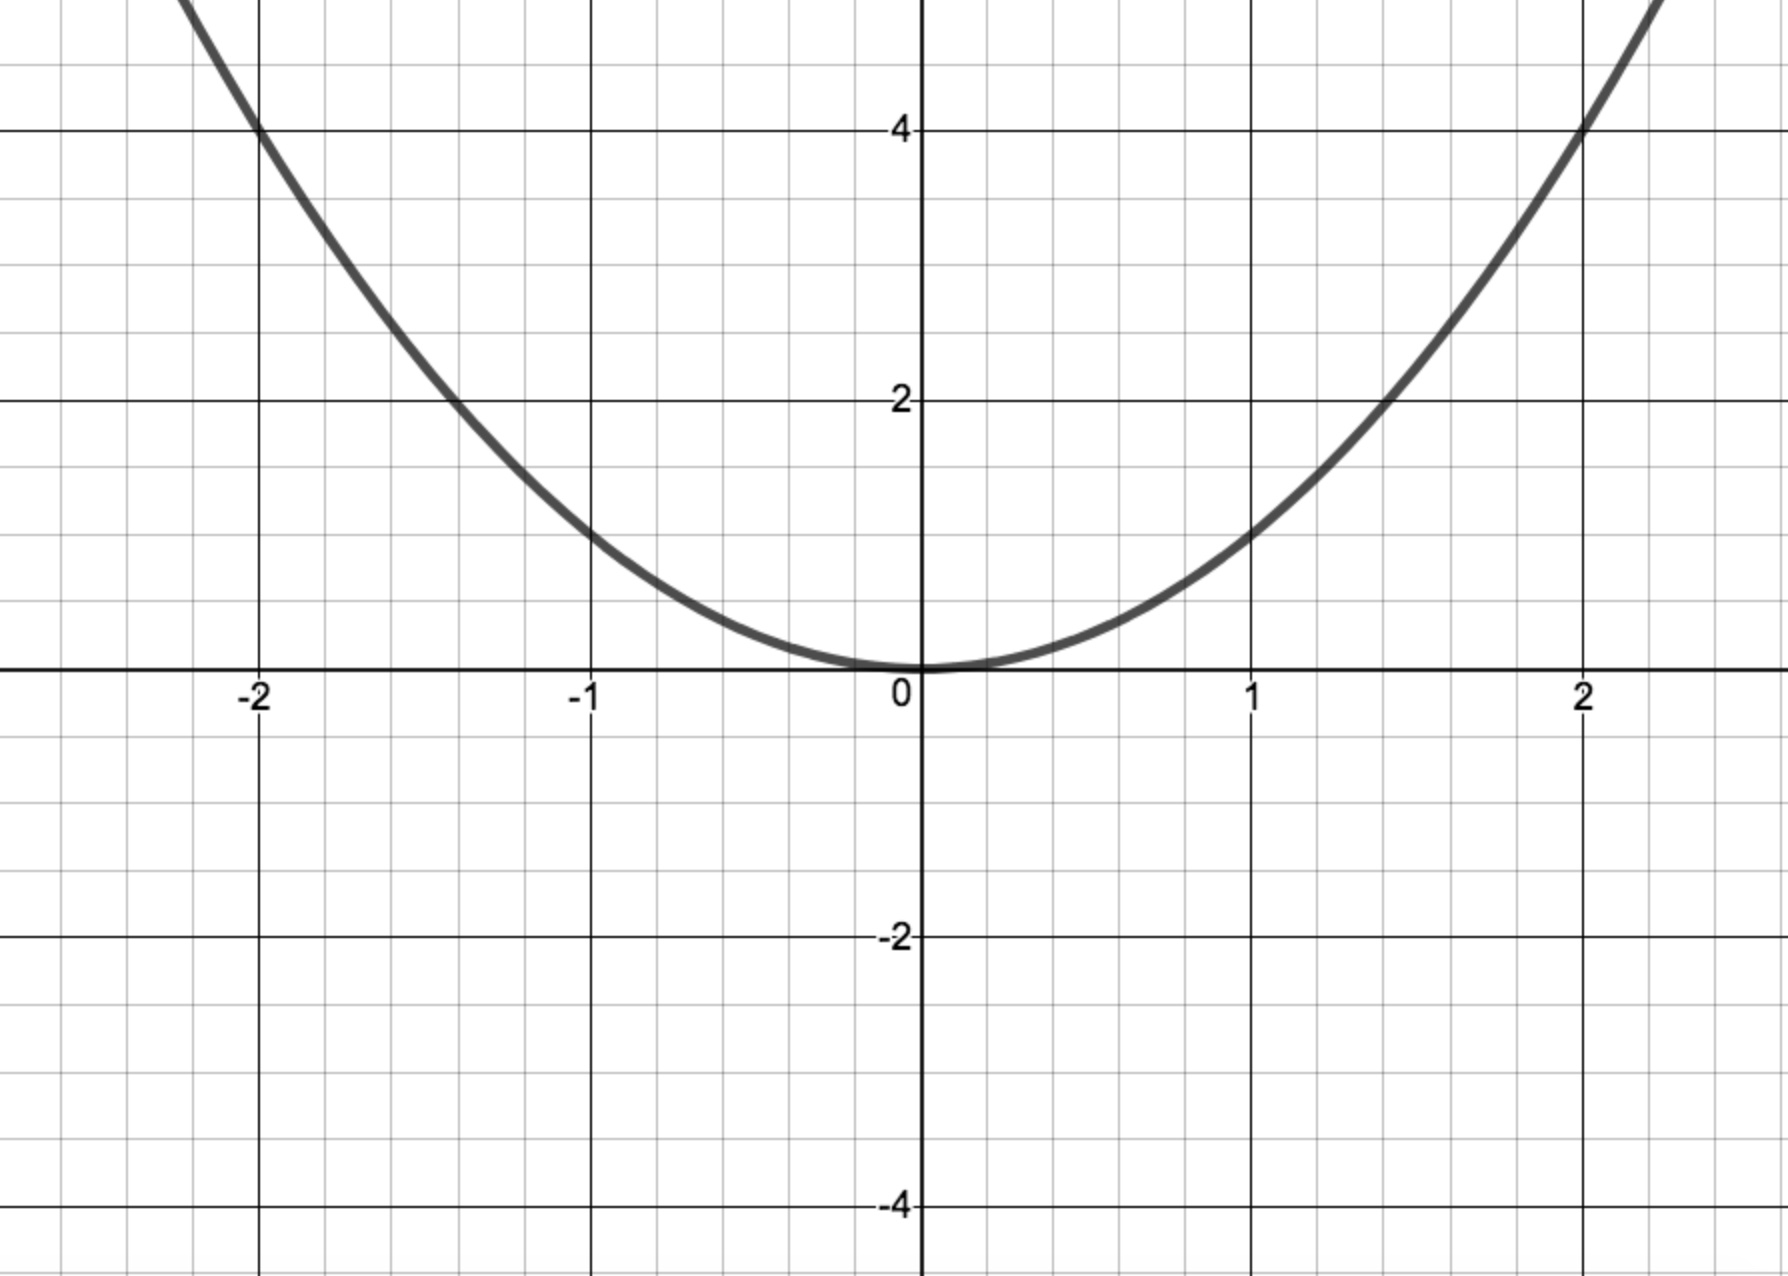
\includegraphics[width=2.75in]{./IntroductiontoDerivativesGraphics/MatchFunc02.jpeg}

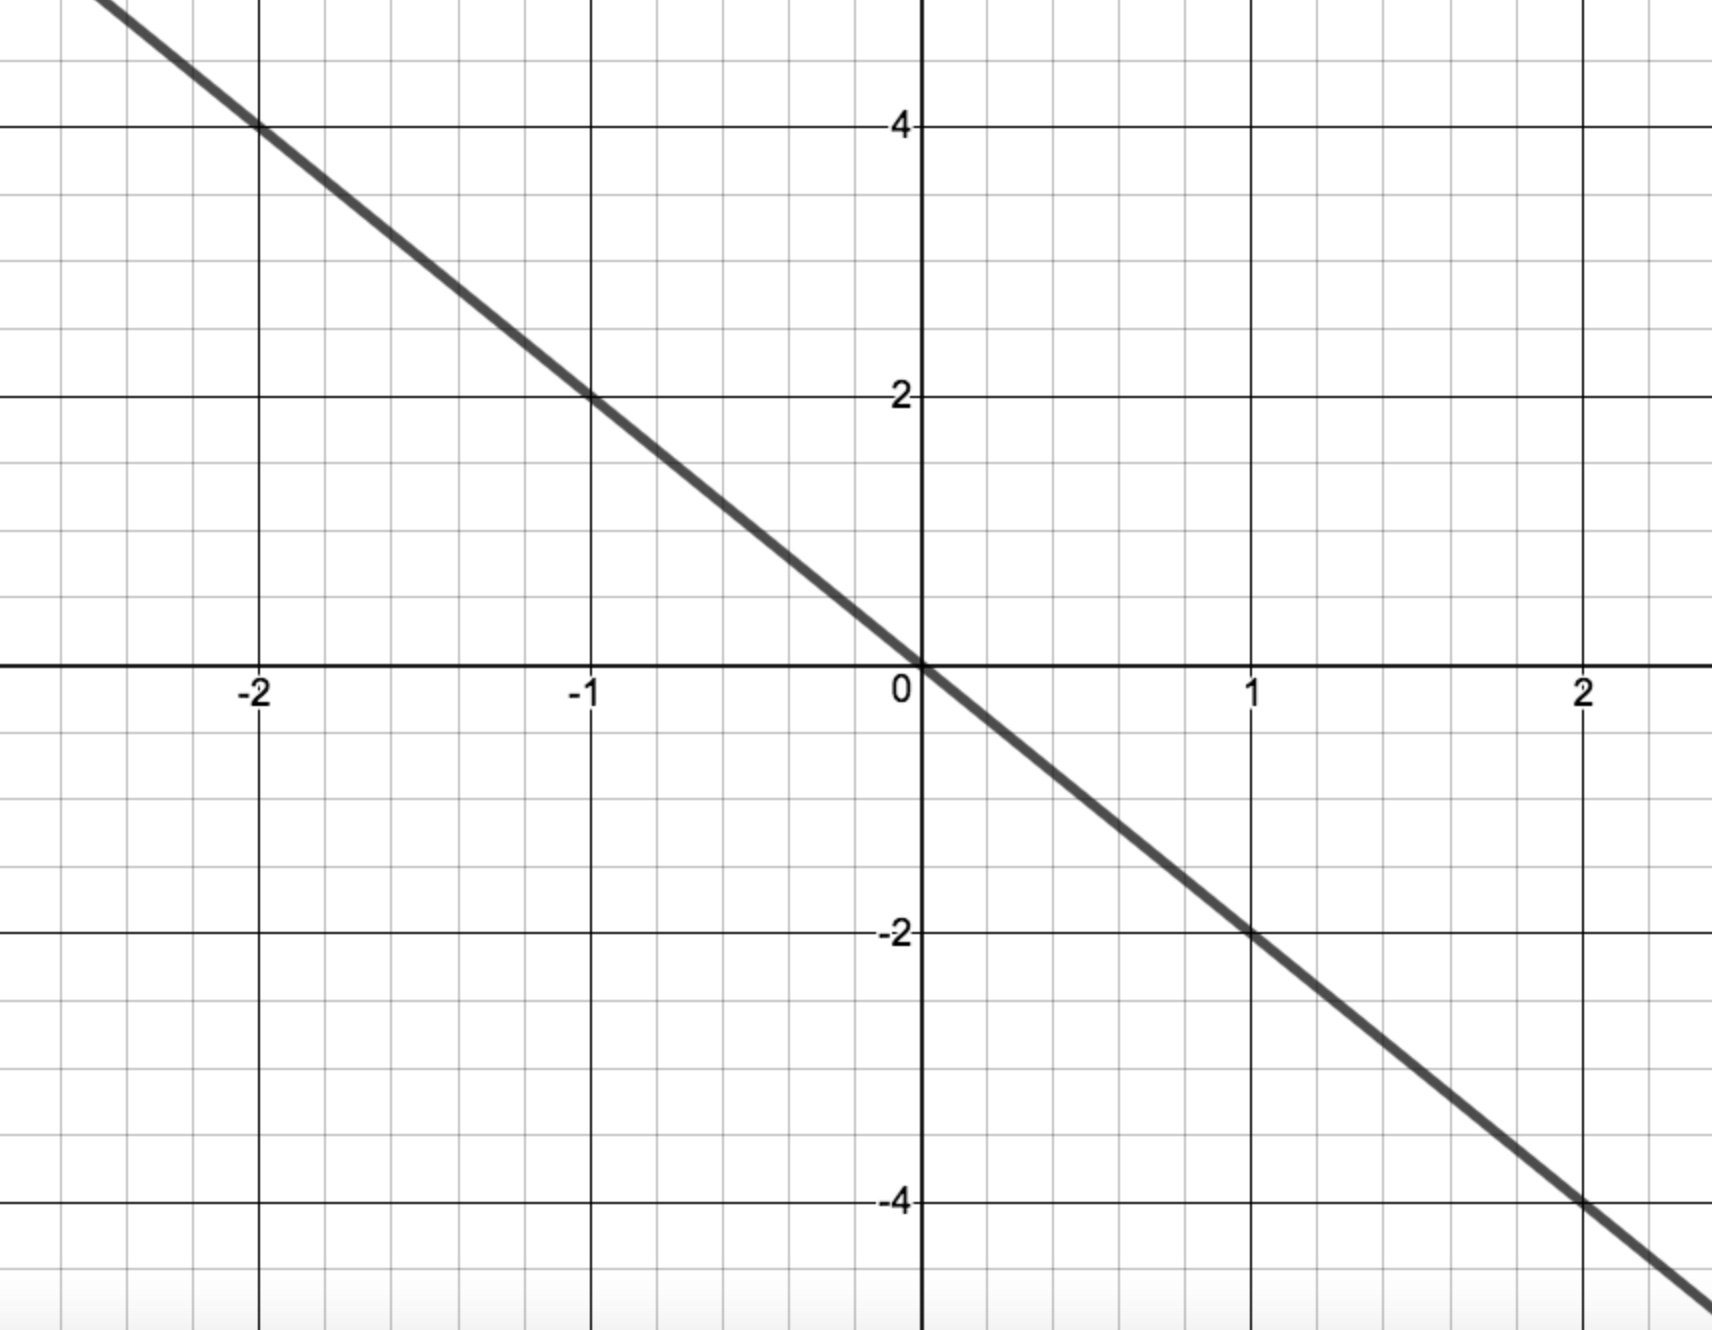
\includegraphics[width=2.75in]{./IntroductiontoDerivativesGraphics/MatchDeriv01.jpeg}

\end{multicols}


\begin{multicols}{2}

\begin{enumerate}
\setcounter{enumi}{\value{HW}}

\item \label{MatchFcnDerivative1last} $y = h(x)$:

\setcounter{HW}{\value{enumi}}
\end{enumerate}


Graph C:

\end{multicols}




\begin{multicols}{2}

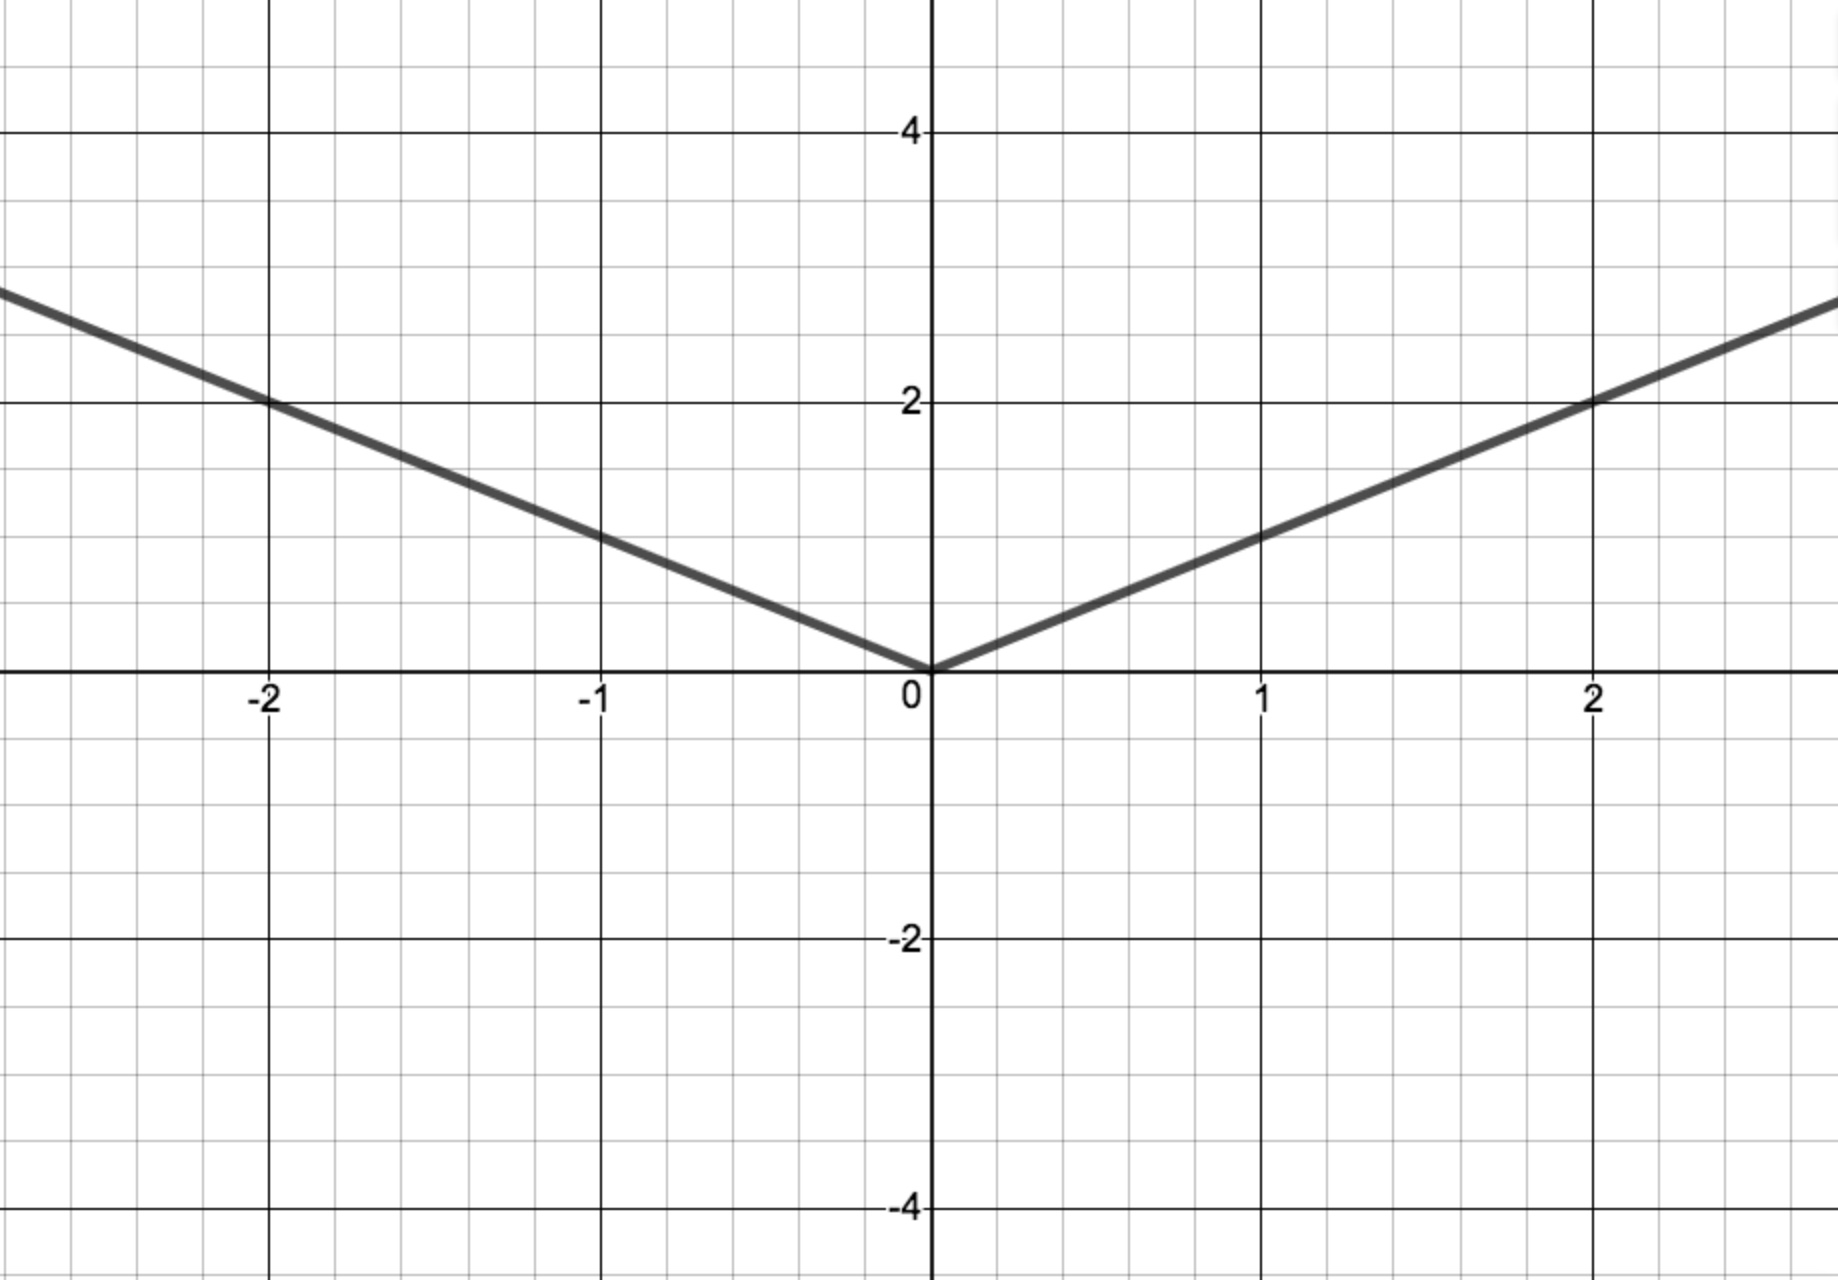
\includegraphics[width=2.75in]{./IntroductiontoDerivativesGraphics/MatchFunc03.jpeg}

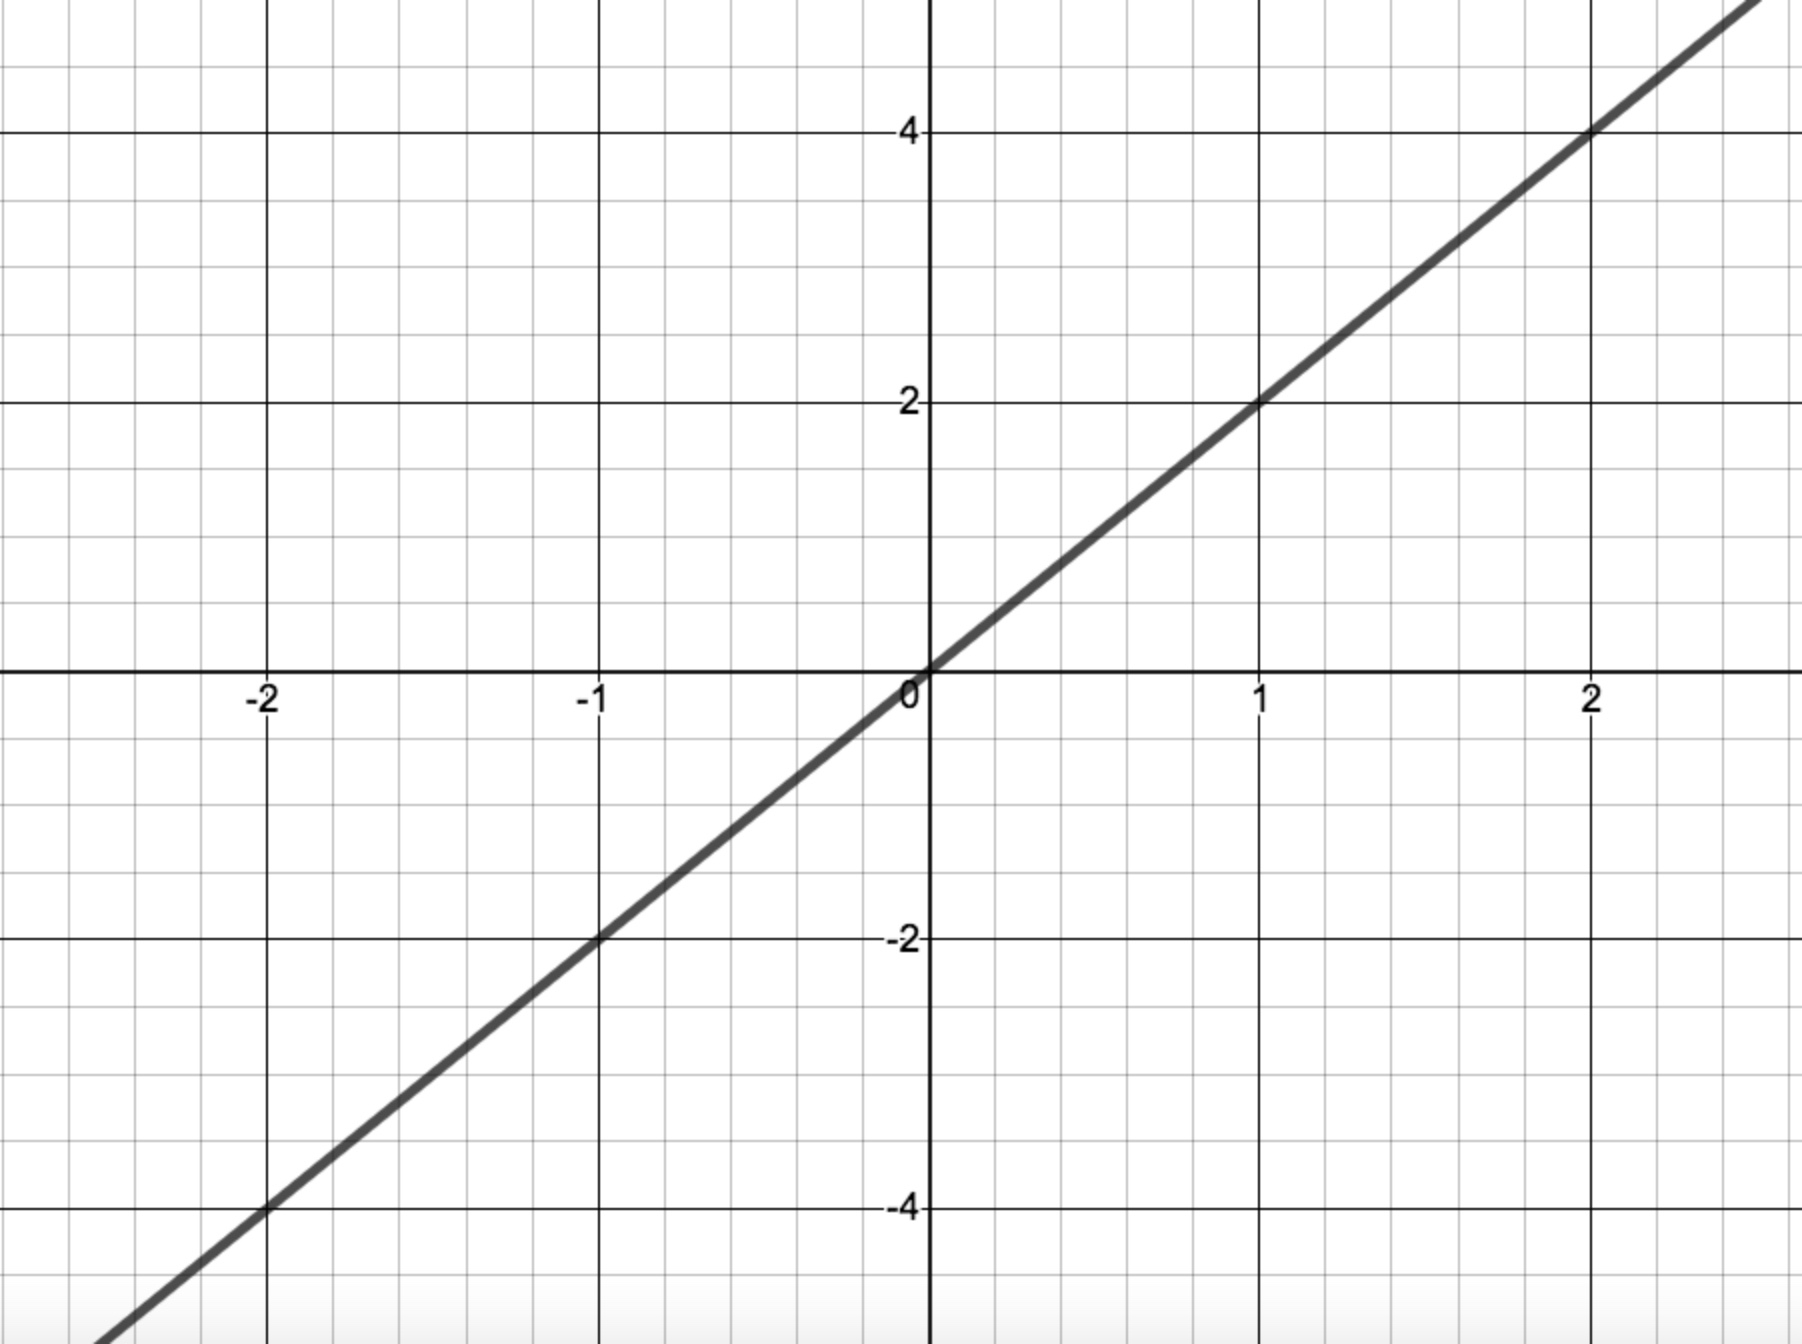
\includegraphics[width=2.75in]{./IntroductiontoDerivativesGraphics/MatchDeriv02.jpeg}

\end{multicols}


\end{center}

In Exercises \ref{MatchFcnDerivative2first} - \ref{MatchFcnDerivative2last}, match the graph of the function with a plausible graph of its derivative.


\begin{center}


\begin{multicols}{2}

\begin{enumerate}
\setcounter{enumi}{\value{HW}}

\item \label{MatchFcnDerivative2first} $y = f(x)$:

\setcounter{HW}{\value{enumi}}
\end{enumerate}

Graph A:

\end{multicols}




\begin{multicols}{2}

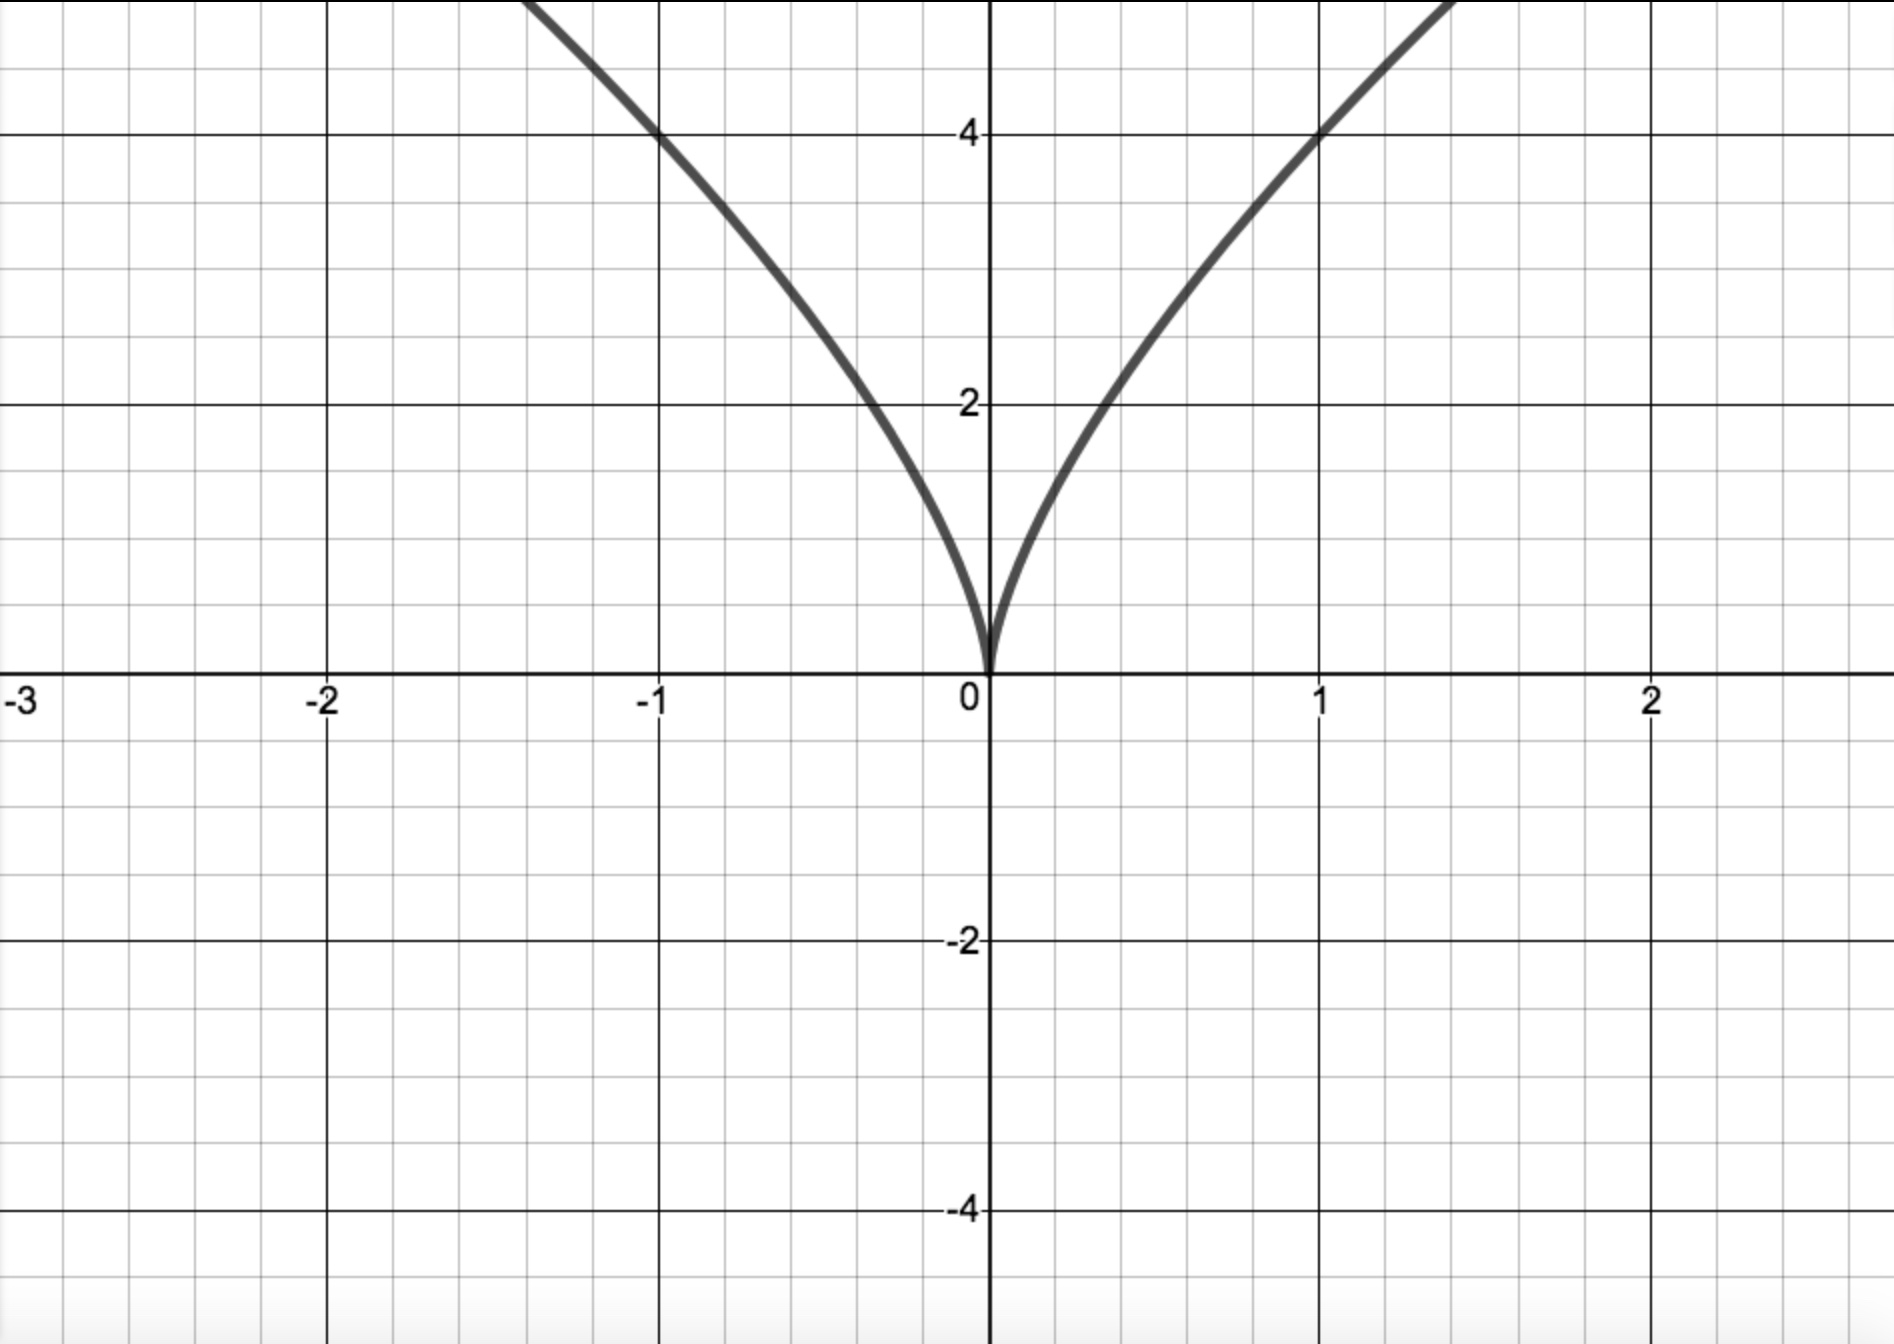
\includegraphics[width=2.75in]{./IntroductiontoDerivativesGraphics/MatchFunc04.jpeg}

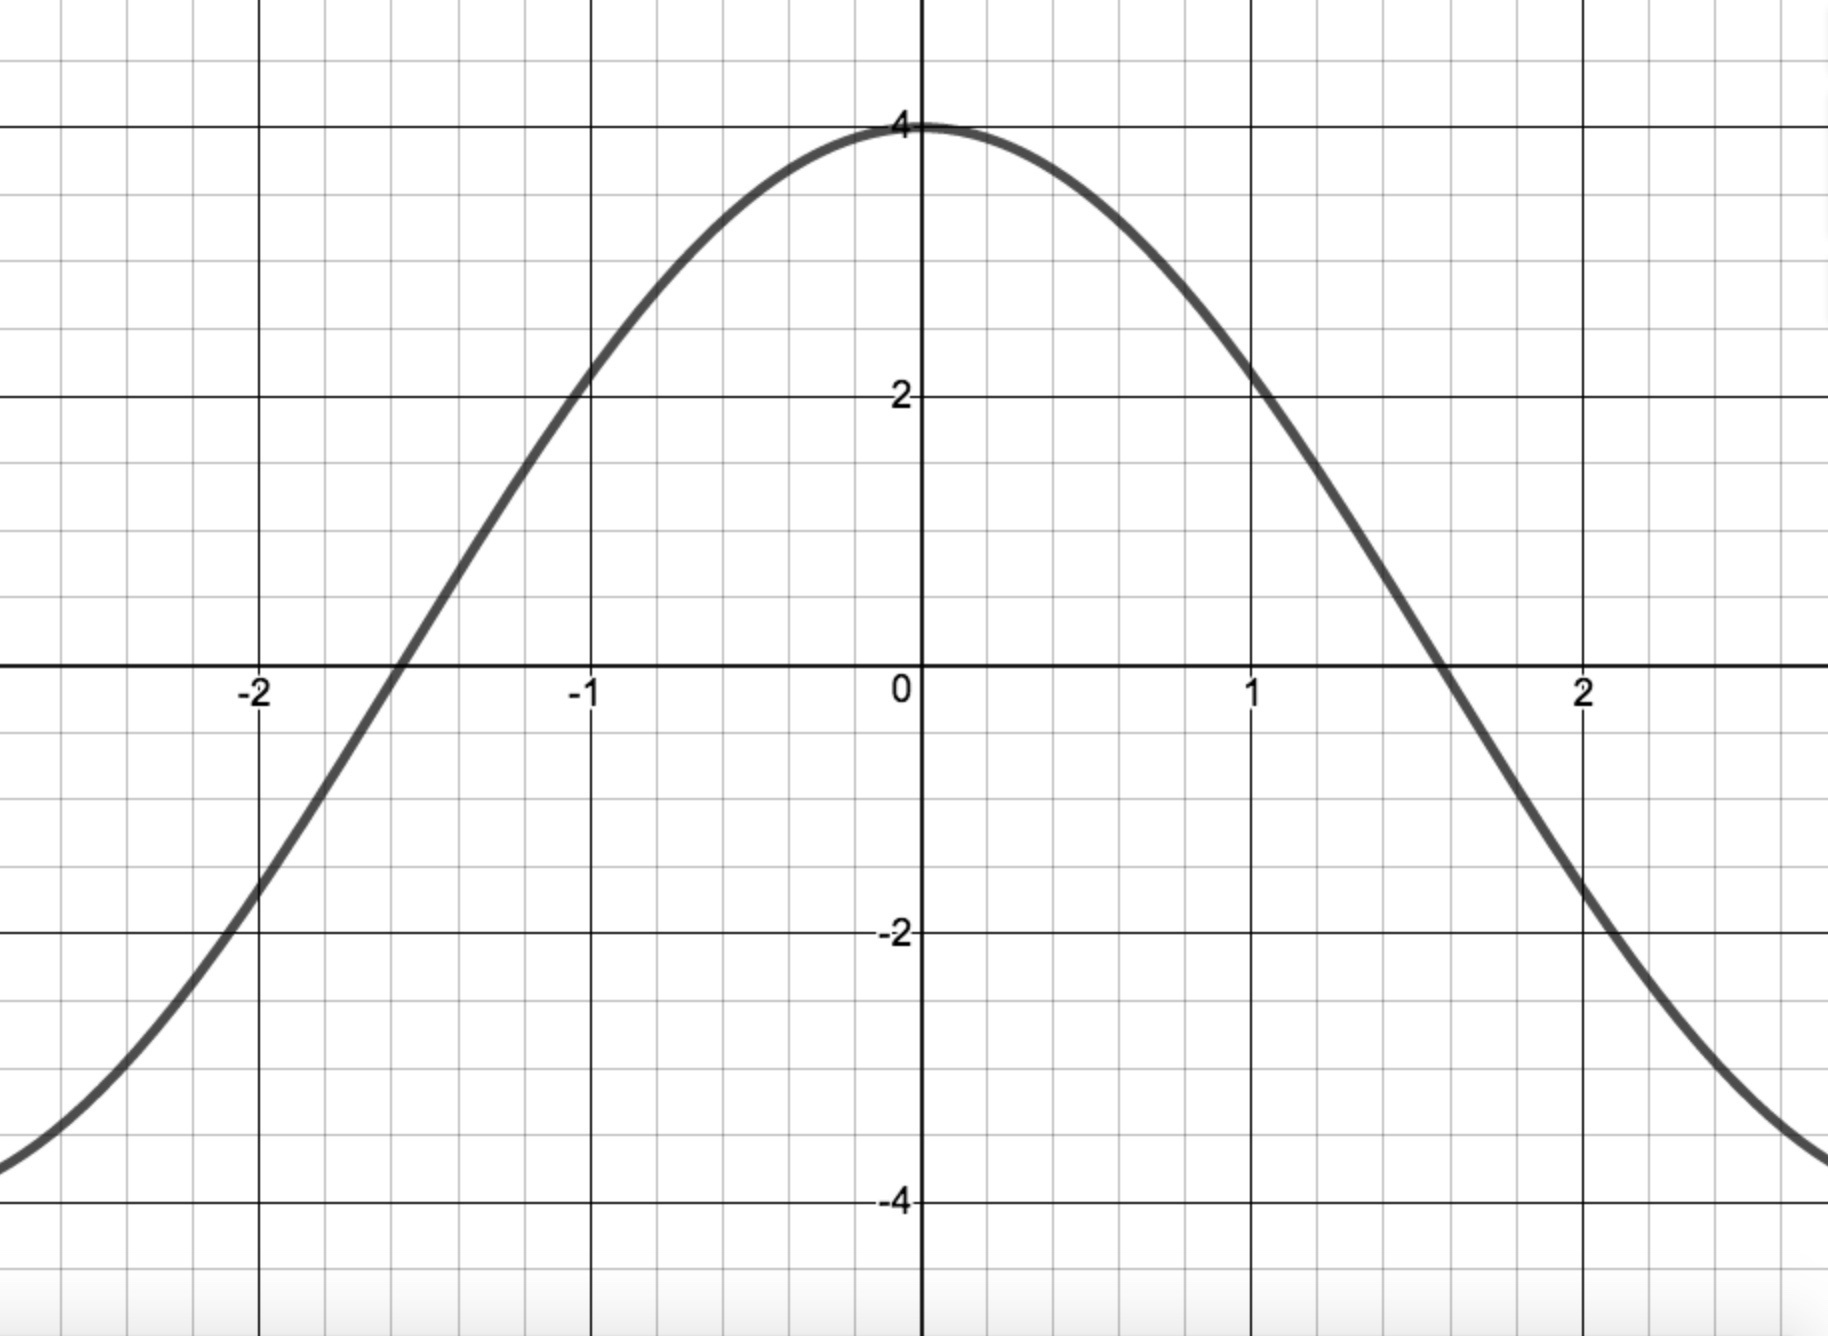
\includegraphics[width=2.75in]{./IntroductiontoDerivativesGraphics/MatchDeriv06.jpeg}

\end{multicols}



\begin{multicols}{2}

\begin{enumerate}
\setcounter{enumi}{\value{HW}}

\item $y = g(x)$:

\setcounter{HW}{\value{enumi}}
\end{enumerate}

Graph B:

\end{multicols}




\begin{multicols}{2}

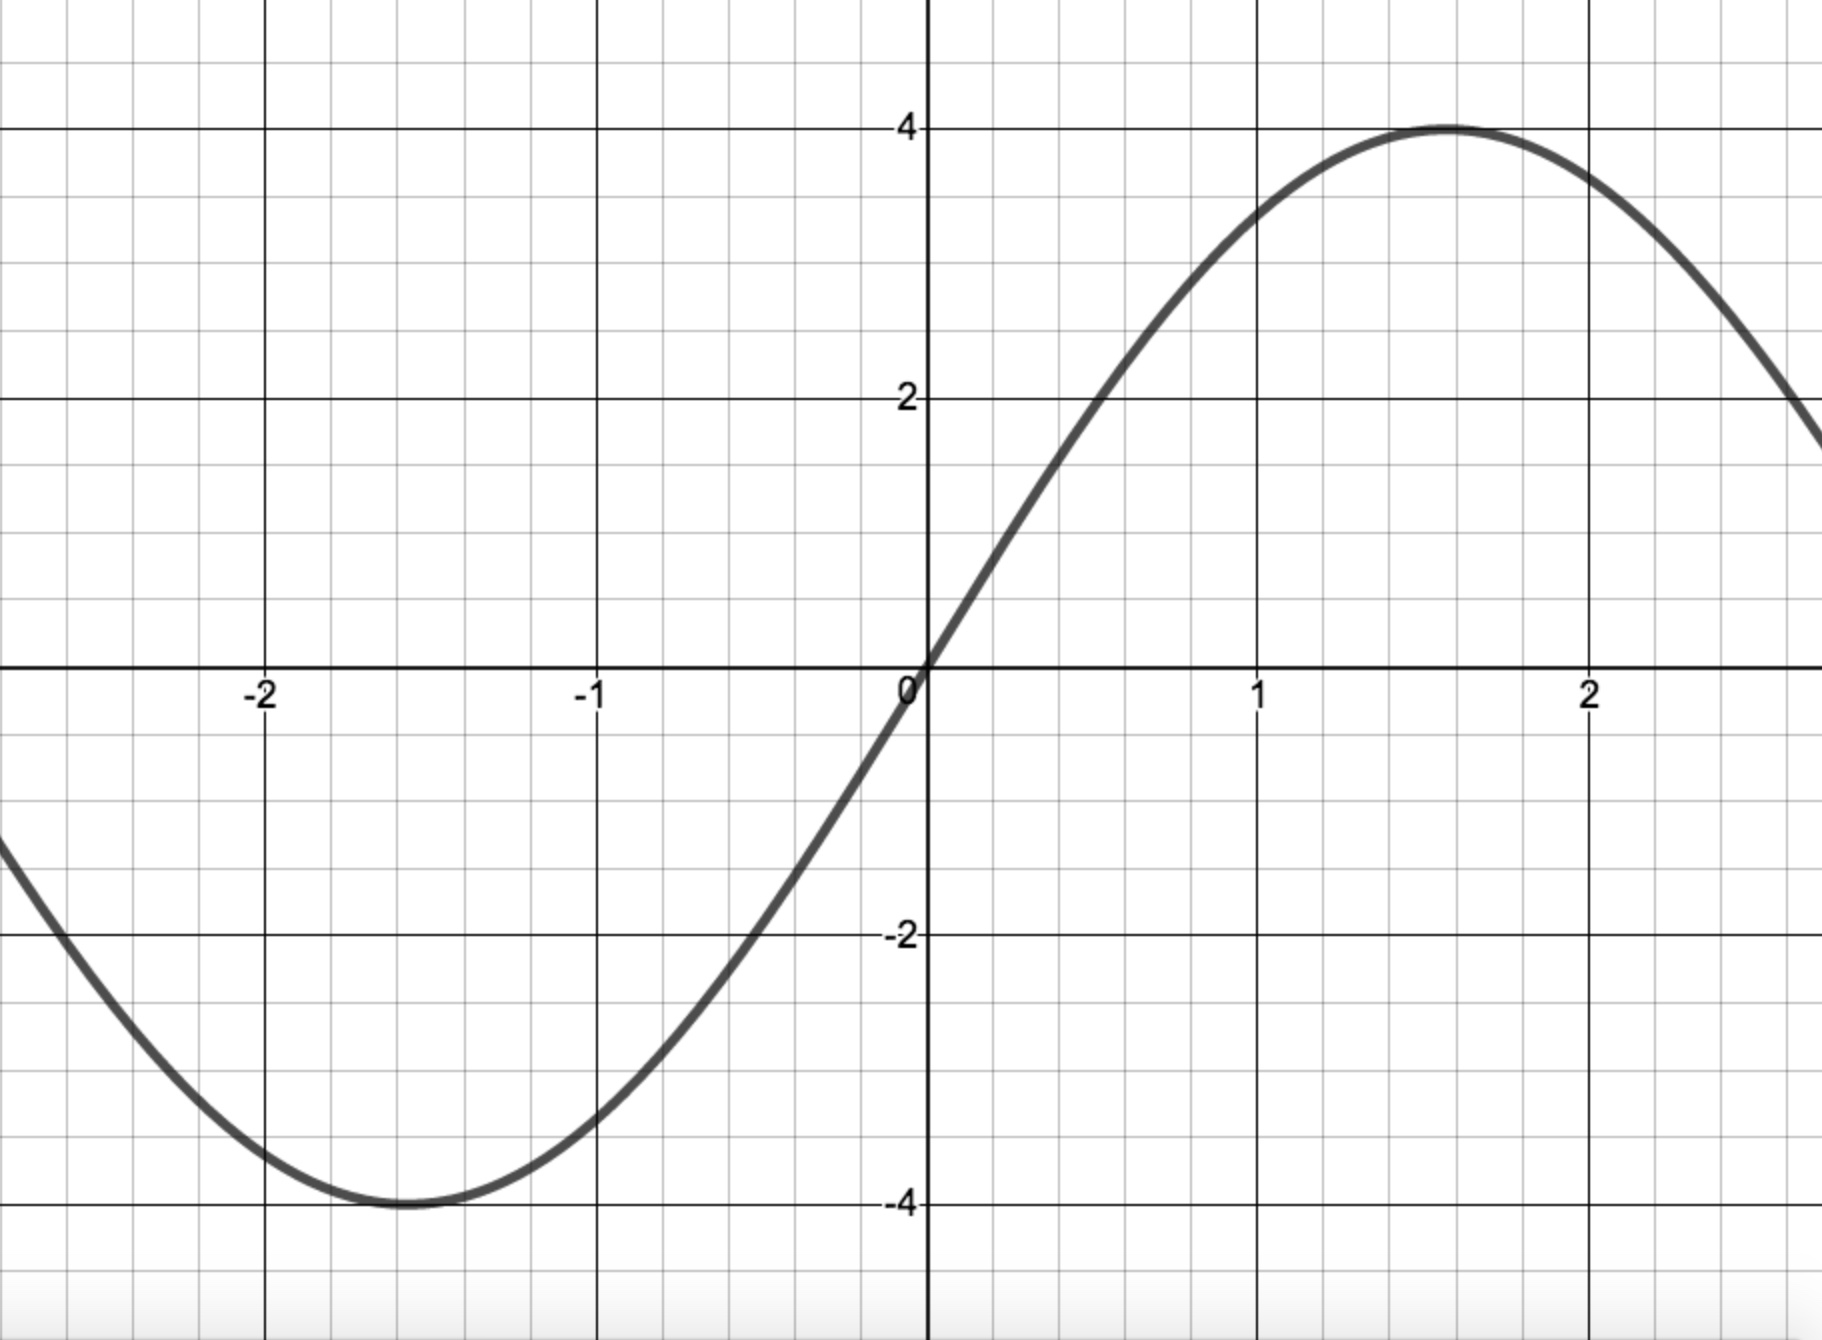
\includegraphics[width=2.75in]{./IntroductiontoDerivativesGraphics/MatchFunc06.jpeg}

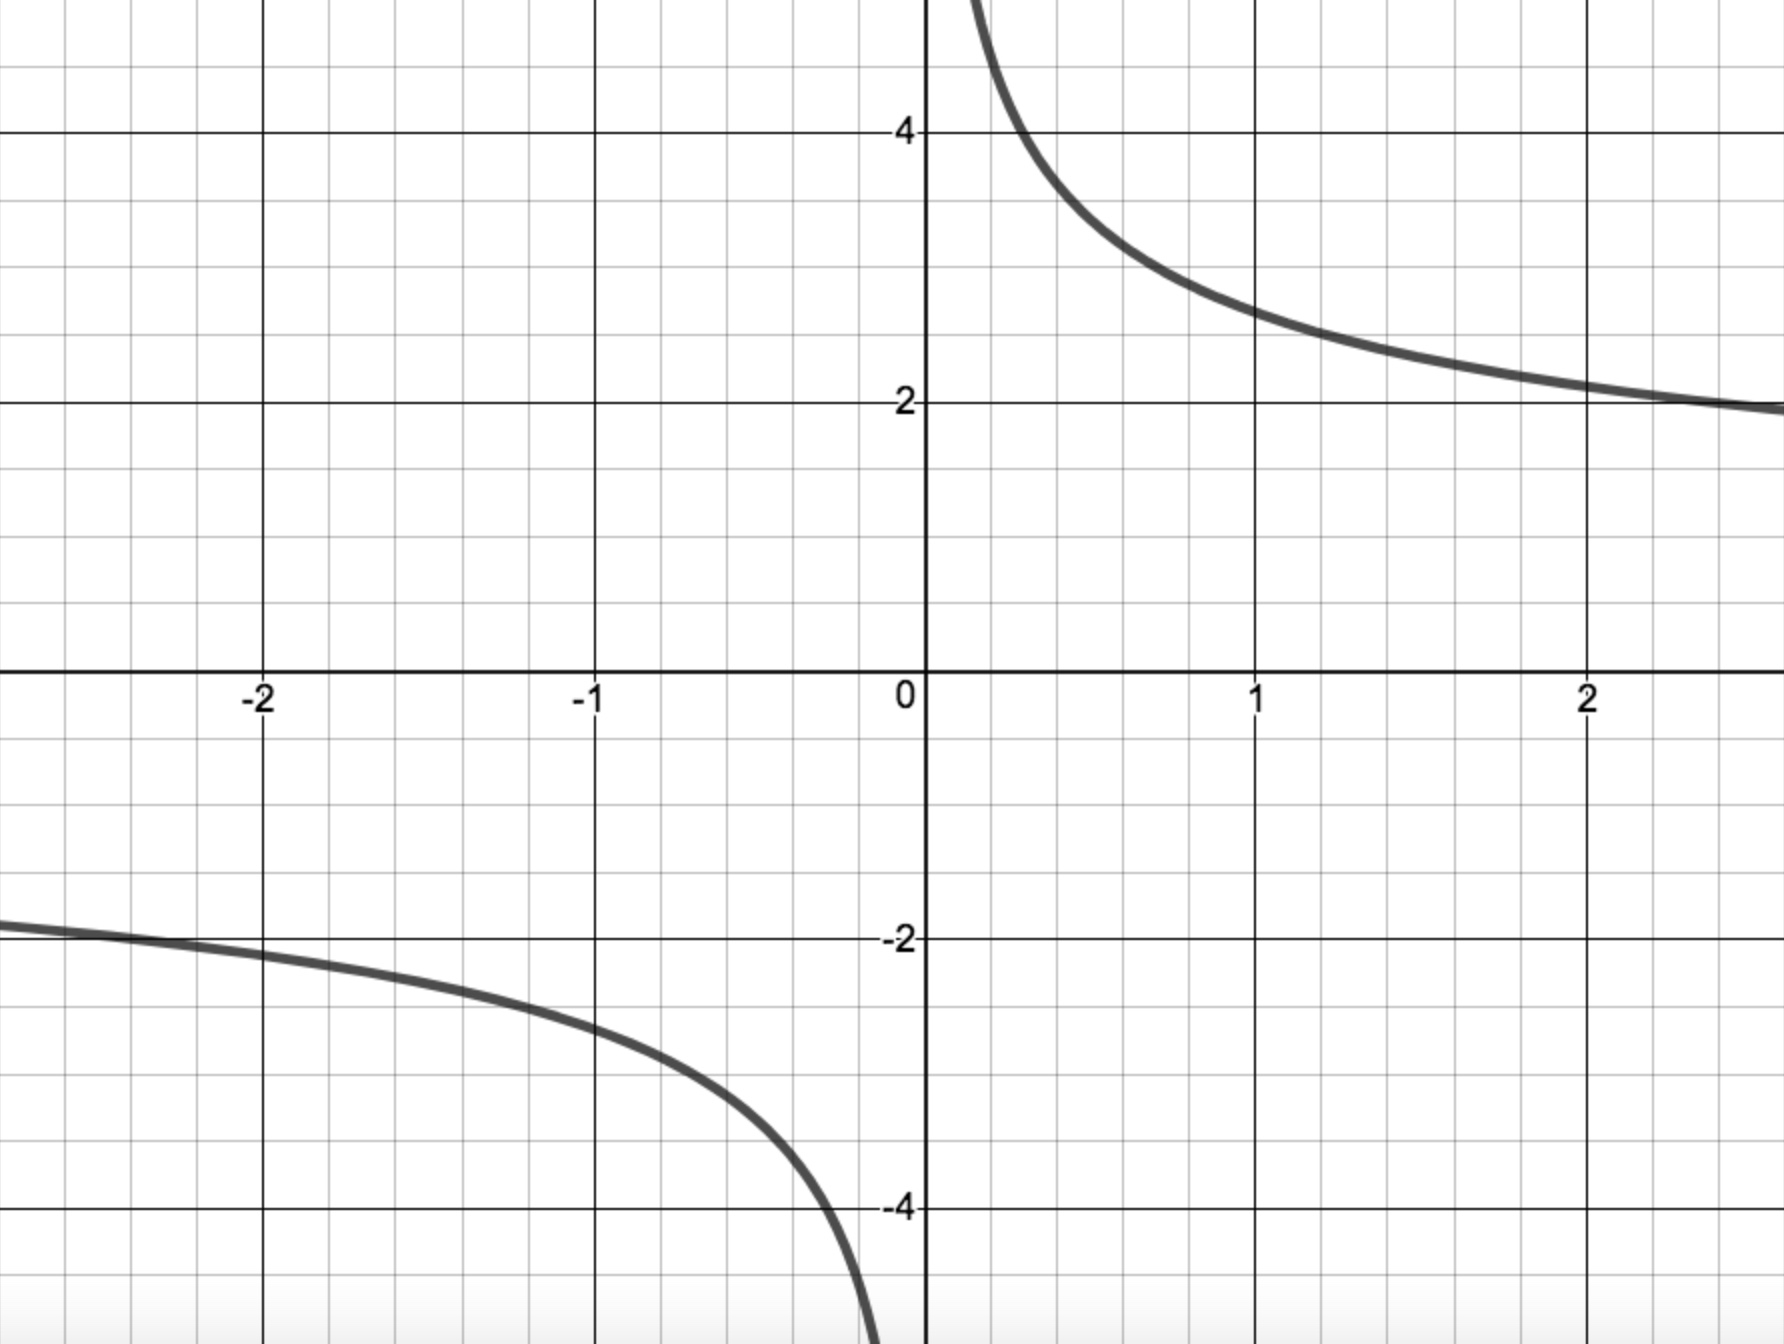
\includegraphics[width=2.75in]{./IntroductiontoDerivativesGraphics/MatchDeriv04.jpeg}

\end{multicols}



\begin{multicols}{2}

\begin{enumerate}
\setcounter{enumi}{\value{HW}}

\item \label{MatchFcnDerivative2last}  $y = h(x)$:

\setcounter{HW}{\value{enumi}}
\end{enumerate}

Graph C:

\end{multicols}



\begin{multicols}{2}

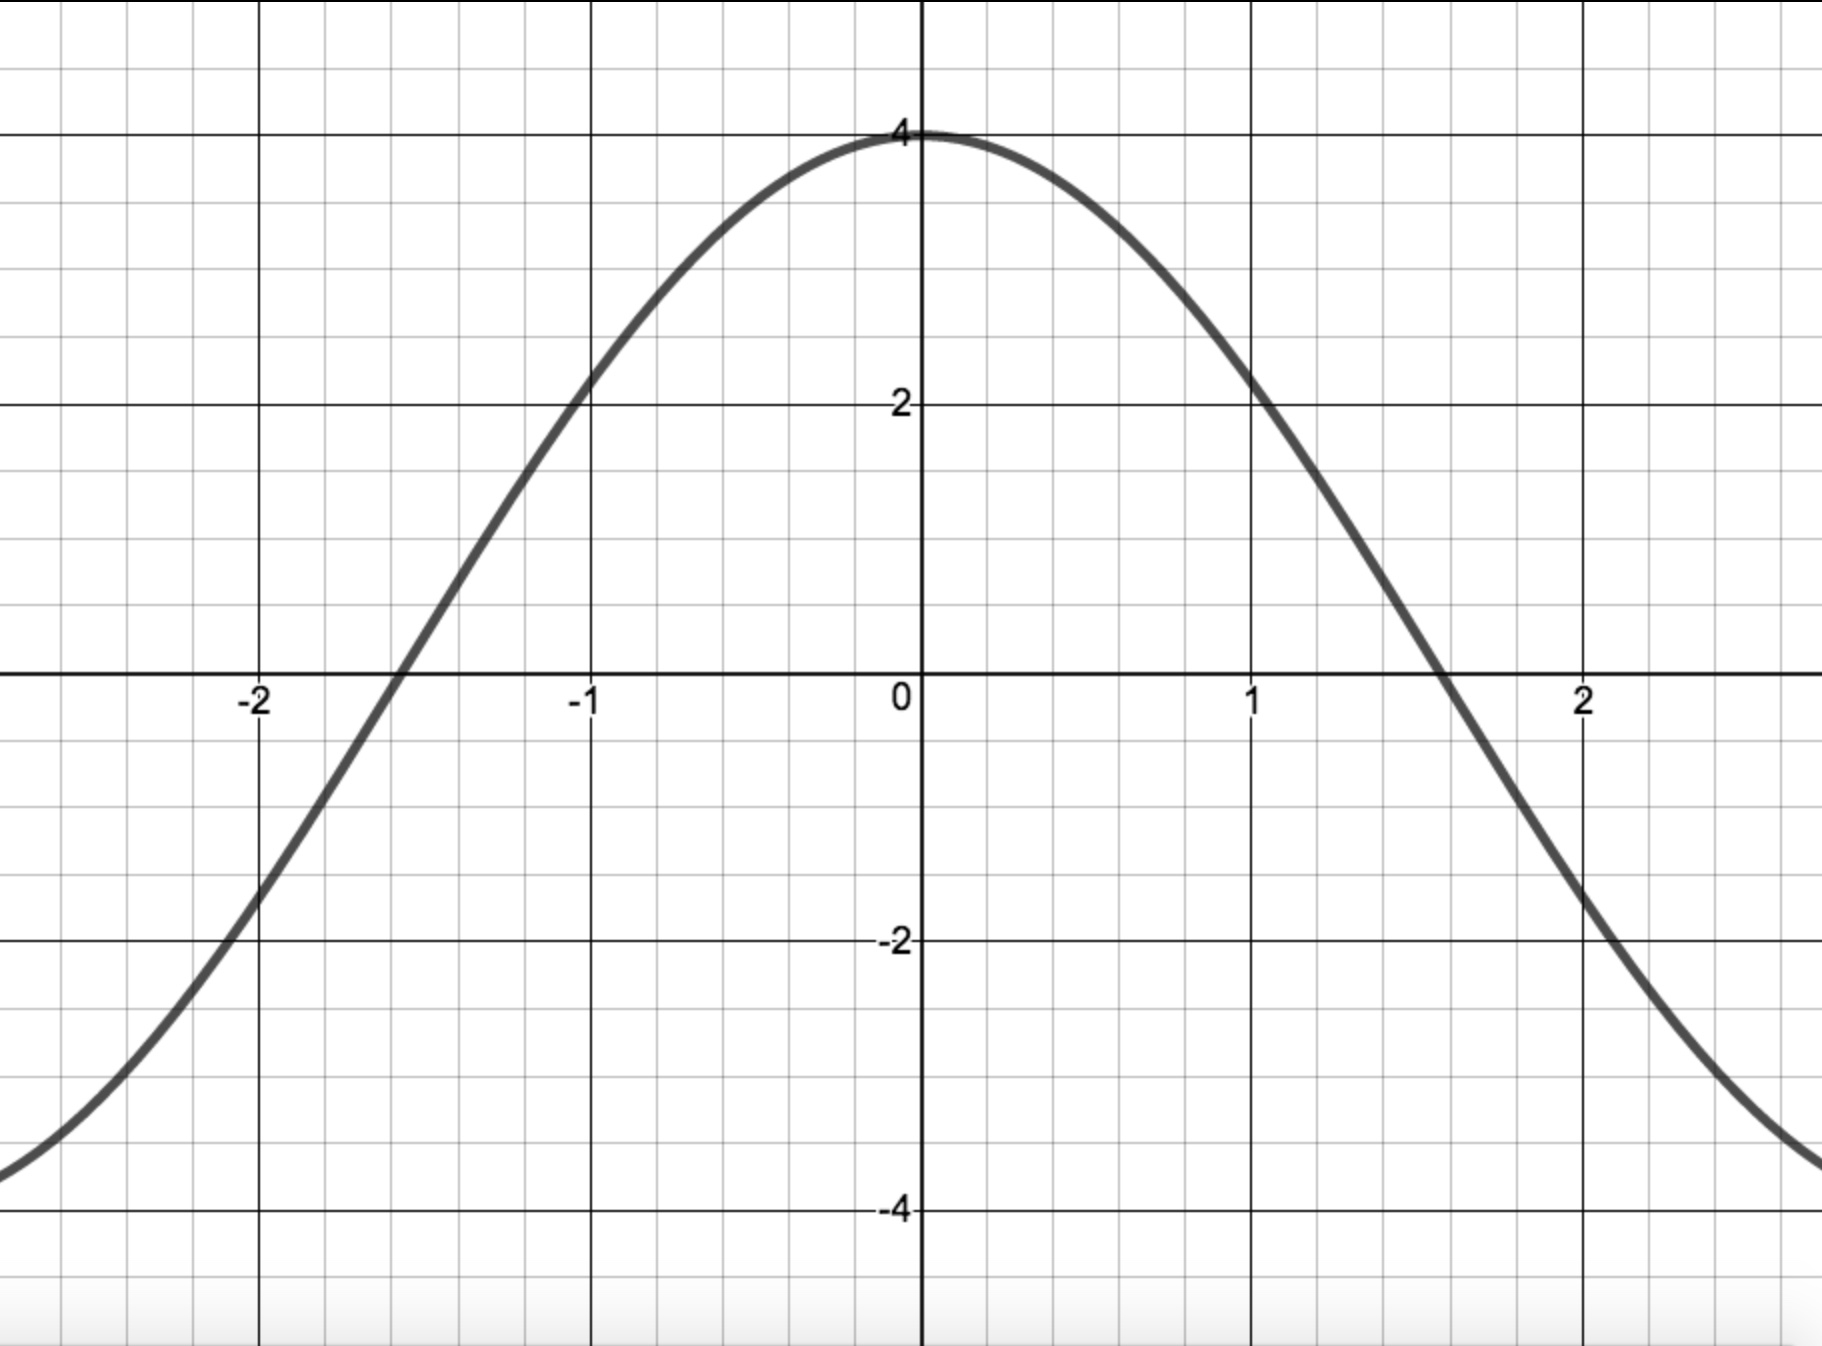
\includegraphics[width=2.75in]{./IntroductiontoDerivativesGraphics/MatchFunc05.jpeg}

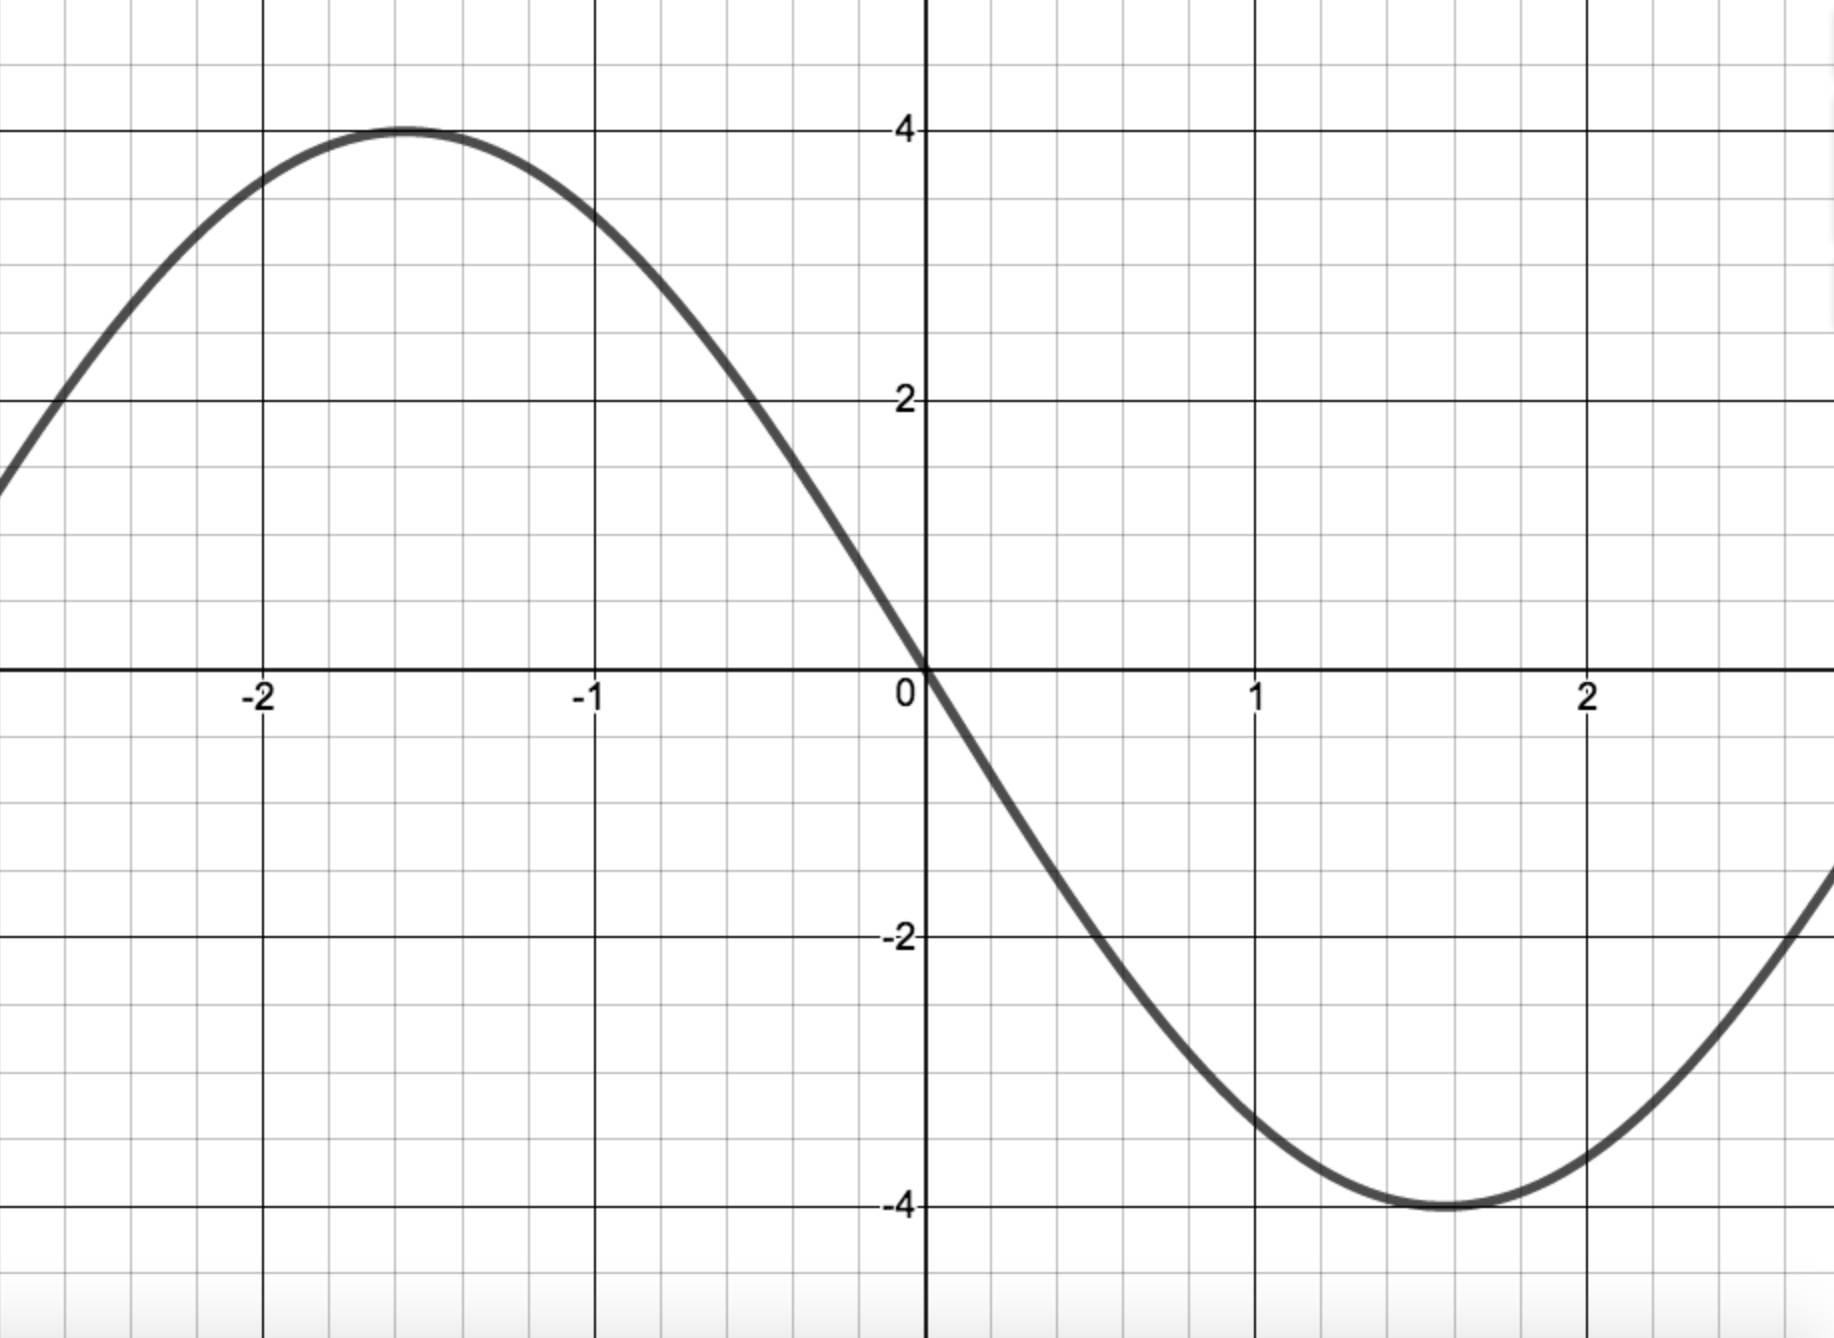
\includegraphics[width=2.75in]{./IntroductiontoDerivativesGraphics/MatchDeriv05.jpeg}

\end{multicols}

\end{center}


\newpage


\subsection{Answers}


\begin{enumerate}

\item $\ds{\lim_{h \rightarrow 0} 2 = 2}$, $\ds{\lim_{h \rightarrow 0} 2 = 2}$
\item $\ds{\lim_{h \rightarrow 0} -3 = -3}$, $\ds{\lim_{h \rightarrow 0} -3 = -3}$,

\setcounter{HW}{\value{enumi}}
\end{enumerate}

\begin{enumerate}
\setcounter{enumi}{\value{HW}}

\item $\ds{\lim_{h \rightarrow 0} 0 = 0}$,  $\ds{\lim_{h \rightarrow 0} 0 = 0}$
\item  $\ds{\lim_{h \rightarrow 0} (3h+11)= 11}$,   $\ds{\lim_{h \rightarrow 0} (6x+3h-1)= 6x-1}$

\setcounter{HW}{\value{enumi}}
\end{enumerate}

\begin{enumerate}
\setcounter{enumi}{\value{HW}}

\item    $\ds{\lim_{h \rightarrow 0} (-h-2) = -2}$,   $\ds{\lim_{h \rightarrow 0} (-2x-h+2) = -2x+2}$   
\item   $\ds{\lim_{h \rightarrow 0} (4h+16) = 16}$,   $\ds{\lim_{h \rightarrow 0} (8x+4h) = 8x}$ 

\setcounter{HW}{\value{enumi}}
\end{enumerate}

\begin{enumerate}
\setcounter{enumi}{\value{HW}}

\item \begin{itemize}  \item $f'(2) = \ds{\lim_{h \rightarrow 0} (-h-3) = -3}$

\smallskip

\item  $y = f'(2)(x-2) + f(2) = (-3)(x-2)+(-2)$ so $y  = -3x+4$.

\smallskip

\item   $f'(x) =  \ds{\lim_{h \rightarrow 0} (-2x-h+1) = -2x+1}$ 

\smallskip

\item  $y = f'(0)(x-0) + f(0) = (1)(x-0) + 0$ so $y = x$.

\smallskip

\end{itemize}

\item \begin{itemize}

\item $f'(2) = \ds{\lim_{h \rightarrow 0} \left( h^2+6h+12 \right) = 12}$

\smallskip

\item  $y = f'(2)(x-2) + f(2) = 12(x-2)+ 9$ so $y = 12x - 15$.

\smallskip

\item  $f'(x) = \ds{\lim_{h \rightarrow 0} \left(3x^{2} + 3xh + h^{2} \right) = 3x^{2}}$ 

\smallskip

\item $y = f'(0)(x-0)+f(0) = 0(x-0)+1$ so $y = 1$.

\smallskip

\end{itemize} 

\setcounter{HW}{\value{enumi}}
\end{enumerate}

\begin{enumerate}
\setcounter{enumi}{\value{HW}}

\item  $f'(x) = \ds{\lim_{h \rightarrow 0} m= m}$.

\item  \begin{itemize} \item  $f'(x) = \ds{\lim_{h \rightarrow 0} (2ax + ah + b) = 2ax + b}$.

\smallskip

\item  Solving $f'(x) = 2ax + b = 0$ for $x$ gives $x = -\frac{b}{2a}$ which is the formula for the $x$-coordinate of the vertex of the parabola $y = f(x)$.  If we zoom in near the the vertex of a parabola, the graph becomes locally flat so it makes sense the slope of the tangent line,  $f'(x) = 0$ there. 

\end{itemize} 

\setcounter{HW}{\value{enumi}}
\end{enumerate}

\begin{enumerate}
\setcounter{enumi}{\value{HW}}

\item  $\ds{ \lim_{\Delta x \rightarrow 0} \dfrac{2}{\Delta x-1} = -2}$,   $\ds{ \lim_{\Delta x \rightarrow 0} \dfrac{-2}{x(x+\Delta x)} = - \dfrac{2}{x^2}}$
 
\item  $\ds{ \lim_{\Delta x \rightarrow 0} \dfrac{-3}{2(\Delta x - 2)} = \dfrac{3}{4}}$,   $\ds{ \lim_{\Delta x \rightarrow 0} \dfrac{3}{(x+\Delta x-1)(x-1)} =  \dfrac{3}{(x-1)^2}}$  

\setcounter{HW}{\value{enumi}}
\end{enumerate}

\begin{enumerate}
\setcounter{enumi}{\value{HW}}

\item   $\ds{ \lim_{\Delta x \rightarrow 0} \dfrac{2-\Delta x}{(\Delta x - 1)^2} =2}$,   $\ds{ \lim_{\Delta x \rightarrow 0}\dfrac{-(2x+\Delta x)}{x^2(x+\Delta x)^2} =  - \dfrac{2}{x^3}}$   

\item    $\ds{ \lim_{\Delta x \rightarrow 0} \dfrac{-1}{2(\Delta x+4)} = - \dfrac{1}{8}}$,   $\ds{ \lim_{\Delta x \rightarrow 0} \dfrac{-2}{(x+5)(x+\Delta x+5)}=  - \dfrac{2}{(x+5)^2}}$    

\setcounter{HW}{\value{enumi}}
\end{enumerate}

\begin{enumerate}
\setcounter{enumi}{\value{HW}}

\item \begin{itemize}

\item  $f'(-1) =\ds{ \lim_{\Delta x \rightarrow 0} \dfrac{4}{7(4 \Delta x - 7)} = - \dfrac{4}{49}}$

\smallskip

\item $y = f'(-1)(x-(-1)) + f(-1) = -\frac{4}{49}(x + 1) + \left(-\frac{1}{7}\right)$ so $y = -\frac{4}{49} \, x - \frac{11}{49}$.   

\smallskip

\item  $f'(x) = \ds{ \lim_{\Delta x \rightarrow 0} \dfrac{-4}{(4x-3)(4x+4\Delta x-3)} =  - \dfrac{4}{(4x-3)^2}}$  

\smallskip

\item $y = f'(0)(x-0)+f(0) = -\frac{4}{9} (x-0) + \left(-\frac{1}{3}\right)$ so $y = -\frac{4}{9} \, x - \frac{1}{3}$.

\smallskip

\end{itemize}
   
\item \begin{itemize}

\item  $f'(-1) = \ds{ \lim_{\Delta x \rightarrow 0} \dfrac{6}{\Delta x + 1}= 6}$

\smallskip

\item $y = f'(-1)(x-(-1)) + f(-1) = 6(x+1) + (-3)$ so $y = 6x+3$.

\smallskip

\item  $f'(x) =\ds{ \lim_{\Delta x \rightarrow 0} \dfrac{6}{(x+2)(x+\Delta x+2)} =   \dfrac{6}{(x+2)^2}}$ 

\smallskip    

\item  $y = f'(0)(x-0) + f(0) = \frac{3}{2} \, (x-0)+0$ so $y = \frac{3}{2} \, x$.


\smallskip


\end{itemize}

 
\setcounter{HW}{\value{enumi}}
\end{enumerate}

\begin{enumerate}
\setcounter{enumi}{\value{HW}}

\item   \begin{itemize}

\item  $f'(-1) = \ds{ \lim_{\Delta x \rightarrow 0} \dfrac{9}{10(\Delta x - 10)} = -\dfrac{9}{100}}$

\smallskip

\item $y = f'(-1)(x-(-1)) + f(-1) = -\frac{9}{100} \, (x+1) + \frac{1}{10}$ so $y = - \frac{9}{100} \, x + \frac{1}{100}$.

\smallskip

\item  $f'(x) =\ds{ \lim_{\Delta x \rightarrow 0} \dfrac{-9}{(x - 9)(x + \Delta x - 9)} =   -\dfrac{9}{(x-9)^2}}$   

\smallskip  

\item  $y = f'(0)(x-0) + f(0) = -\frac{1}{9} \, (x-0)+0$ so $y = -\frac{1}{9} \, x$.

\smallskip

\end{itemize}

\item \begin{itemize}  

\item  $f'(-1) = \ds{ \lim_{\Delta x \rightarrow 0} \dfrac{\Delta x}{2 \Delta x - 1} = 0}$

\smallskip

\item $y = f'(-1)(x-(-1)) + f(-1) = (0) (x+1) + (-1)$ so $y = -1$.

\smallskip

\item  $f'(x) =\ds{ \lim_{\Delta x \rightarrow 0}\dfrac{2x^2+2x\Delta x+2x+\Delta x}{(2x+1)(2x+2\Delta x+1)}=  \dfrac{2x^2+2x}{(2x+1)^2}}$

\smallskip

\item  $y = f'(0)(x-0) + f(0) = (0)(x-0)+0$ so $y = 0$.

\smallskip

\end{itemize}


\setcounter{HW}{\value{enumi}}
\end{enumerate}

\begin{enumerate}
\setcounter{enumi}{\value{HW}}

\item  $\ds{ \lim_{\Delta t \rightarrow 0}\dfrac{-1}{\sqrt{9-\Delta t} +3}  = -\dfrac{1}{6}}$,   $\ds{ \lim_{\Delta t \rightarrow 0} \dfrac{-1}{\sqrt{9-t-\Delta t} + \sqrt{9-t}}=   -\dfrac{1}{2 \sqrt{9-t}}}$   
\item  $\ds{ \lim_{\Delta t \rightarrow 0}\dfrac{2}{\sqrt{2\Delta t+1} + 1}  =1}$,   $\ds{ \lim_{\Delta t \rightarrow 0}\dfrac{2}{\sqrt{2t+2\Delta t+1} + \sqrt{2t+1}}=   \dfrac{2}{2 \sqrt{2t+1}}}$    

\setcounter{HW}{\value{enumi}}
\end{enumerate}

\begin{enumerate}
\setcounter{enumi}{\value{HW}}

\item \begin{itemize}

\item  $g'(0) = \ds{ \lim_{\Delta t \rightarrow 0} \dfrac{-4}{\sqrt{5-4\Delta t} + \sqrt{5}}  = - \dfrac{2}{\sqrt{5}}}$

\smallskip

\item  $y = g'(0) (x - 0) + g(0) =  -\frac{2}{\sqrt{5}} \, (x-0) + \sqrt{5}$ so $y = -\frac{2}{\sqrt{5}} \, x + \sqrt{5}$.

\smallskip

\item  $g'(t) =  \ds{ \lim_{\Delta t \rightarrow 0} \dfrac{-4}{\sqrt{-4t-4\Delta t+5} + \sqrt{-4t+5}} =   -\dfrac{2}{\sqrt{-4t+5}}}$

\smallskip

\item  $y = g'(1)(x-1)+g(1) = (-2)(x-1) + 1$ so $y = -2x+3$.

\smallskip

\end{itemize}

\item   \begin{itemize}

\item  $g'(0) = \ds{ \lim_{\Delta t \rightarrow 0} \dfrac{-1}{\sqrt{4-\Delta t} + 2}  = - \dfrac{1}{4}}$

\smallskip

\item  $y = g'(0) (x - 0) + g(0) =  -\frac{1}{4} \, (x-0) + 2$ so $y = -\frac{1}{4} \, x +2$.

\smallskip

\item  $g'(t) = \ds{ \lim_{\Delta t \rightarrow 0} \dfrac{-1}{\sqrt{4-t-\Delta t} + \sqrt{4-t}} = -\dfrac{1}{2 \sqrt{4-t}} }$  

\smallskip

\item  $y = g'(1)(x-1)+g(1) = -\frac{1}{2 \sqrt{3}} \, (x-1) + \sqrt{3}$ so $y =  -\frac{1}{2 \sqrt{3}}  \, x + \frac{7 \sqrt{3}}{6}$.

\smallskip

\end{itemize}


\item   \begin{enumerate}

\item  If $\Delta t < 0$, then $\sqrt{\Delta t}$ is not a real number.  Hence, $g'(0) = \ds{\lim_{\Delta t \rightarrow 0} \dfrac{g(\Delta t) - g(0)}{\Delta t}}$ does not exist.

\item  $g_{+}'(0) =\ds{ \lim_{\Delta t \rightarrow 0^{+}} (\Delta t)^{\frac{1}{2}}   =  0}$

\smallskip

\item  $y = g_{+}'(0) (x - 0) + g(0) =  (0) (x-0) + 0$ so $y = 0$.  

\smallskip

This line is a tangent line to the graph of $y = t \sqrt{t}$ at $(0,0)$ for $t \geq 0$.

\smallskip

\item  $g'(t) =\ds{ \lim_{\Delta t \rightarrow 0}\dfrac{3t^2+3t\Delta t+(\Delta t)^2}{(t+\Delta t)^{3/2} + t^{3/2}} = \dfrac{3t^2}{2 t^{3/2}} = \dfrac{3}{2} \, t^{1/2}}$ provided $t > 0$.


\end{enumerate}


\setcounter{HW}{\value{enumi}}
\end{enumerate}

\begin{enumerate}
\setcounter{enumi}{\value{HW}}

\item  \begin{enumerate} \item  $g'(t) = \ds{ \lim_{\Delta t \rightarrow 0} \dfrac{a}{\sqrt{at+a\Delta t+b} + \sqrt{at+b}} = \dfrac{a}{2 \sqrt{at+b}} }$.  

\smallskip

\item  We are told $a \neq 0$.  In order for the square roots to be happy, we assume $at + b > 0$.  Hence,   $t >  - \frac{b}{a}$ if $a>0$ and $t < -  \frac{b}{a}$ if $a<0$. 

\end{enumerate}

\setcounter{HW}{\value{enumi}}
\end{enumerate}


\begin{enumerate}
\setcounter{enumi}{\value{HW}}

\item \begin{enumerate} \item  $f$ is continuous at $x=0$ since $\ds{\lim_{x \rightarrow 0} f(x) = \lim_{x \rightarrow 0} |x| = 0 = |0| = f(0)}$.

\smallskip

\item   $\ds{\lim_{h \rightarrow 0^{-}} \dfrac{f(h) - f(0)}{h} = \lim_{h \rightarrow 0^{-}} \dfrac{-h}{h}  =-1}$,  $\ds{\lim_{h \rightarrow 0^{+}} \dfrac{f(h) - f(0)}{h} = \lim_{h \rightarrow 0^{+}} \dfrac{h}{h}  = 1}$

\smallskip
        
\item  Near $x = 0$, the graph of $y = f(x)$ looks like a `$\vee$' shape\footnote{We say the graph of $f$ has a  \index{corner}\textbf{corner} at $(0,0)$ since we have two different, but finite slopes meeting at a point.} consisting of a line of slope $-1$ to the left of $x=0$ and a line with a slope of $+1$ to the right of $x = 0$.

\smallskip

\item  $f'(x) =  \ds{\lim_{h \rightarrow 0} \dfrac{|x+h| - |x|}{h} = -1}$ if $x < 0$ and $f'(x) =  \ds{\lim_{h \rightarrow 0} \dfrac{|x+h| - |x|}{h} = 1}$ of $x > 0$.

\smallskip

\end{enumerate}



\item \begin{enumerate}

\item  $g$ is continuous at $t=0$ since $\ds{\lim_{t \rightarrow 0} g(t) = \lim_{t \rightarrow 0} \sqrt[3]{t} = 0 = \sqrt[3]{0} = g(0)}$.

\smallskip

\item $\ds{\lim_{\Delta t \rightarrow 0} \dfrac{g(\Delta t) - g(0)}{\Delta t} =   \lim_{\Delta t \rightarrow 0} \dfrac{1}{(\Delta t)^{\frac{2}{3}}}   =  \infty}$

\smallskip

        
\item  The graph of $y = g(t)$ near $(0,0)$ is a vertical line.\footnote{We say the graph of $g$ has a  \index{vertical tangent}\index{tangent line ! vertical}\textbf{vertical tangent line} at $(0,0)$.  This is the more formal way to describe all of the `unusual steepness' we saw back in Chapter \ref{RootRadicalPowerFunctions}.}  Since $g$ is increasing through $(0,0)$, the `slope' of this vertical line could be seen as $+ \infty$. 

\smallskip

\item   $g'(t) = \ds{ \lim_{\Delta t \rightarrow 0} \dfrac{1}{(t+\Delta t)^{\frac{2}{3}} + (t+\Delta t)^{\frac{1}{3}} t^{\frac{1}{3}} + t^{\frac{2}{3}}} = \dfrac{1}{3 t^{\frac{2}{3}}} }$, $t \neq 0$.

\end{enumerate}

\item \begin{enumerate}  \item $\ds{\lim_{x \rightarrow 0} h(x) = \lim_{x \rightarrow 0} x^{\frac{2}{3}} = 0 = 0^{\frac{2}{3}} = h(0)}$. 

\item $\ds{\lim_{\Delta x \rightarrow 0^{-}} \dfrac{h(\Delta x) - h(0)}{\Delta x} = \lim_{\Delta x \rightarrow 0^{-}} \dfrac{1}{(\Delta x)^{\frac{1}{3}}} = -\infty}$ and  $\ds{\lim_{\Delta x \rightarrow 0^{+}} \dfrac{h(\Delta x) - h(0)}{\Delta x} = \lim_{\Delta x \rightarrow 0^{+}} \dfrac{1}{(\Delta x)^{\frac{1}{3}}} = \infty}$

\smallskip
        
\item  The graph $y = h(x)$ near $(0,0)$ shows a steeply decreasing graph as we approach $(0,0)$ from the left followed by a steeply increasing graph as we approach $(0,0)$ from the right.\footnote{We say the graph of $f$ has a  \index{cusp}\textbf{cusp} at $(0,0)$ since we have two different, infinite slopes meeting at a point.}

\smallskip

\item  $h'(x) =  \ds{\lim_{\Delta x \rightarrow 0} \dfrac{h(x+\Delta x) - h(x)}{\Delta x} = \lim_{\Delta x \rightarrow 0} \dfrac{2x + \Delta x}{(x+\Delta x)^{\frac{4}{3}} + (x+\Delta x)^{\frac{2}{3}} \, x^{\frac{2}{3}} + x^{\frac{4}{3}}} = \dfrac{2}{3x^{\frac{1}{3}}}}$, $x \neq 0$.
\end{enumerate}

\item  \begin{enumerate}

\item  $v(t) = \ds{\lim_{\Delta t \rightarrow 0} \dfrac{h(t + \Delta t) - h(t)}{\Delta t} = \lim_{\Delta t \rightarrow 0} \dfrac{-16(\Delta t)^2 -32 t \, \Delta t + 22.08 \Delta t}{\Delta t}  = -32t + 22.08}$.

\item   $v(0) = -32(0) + 22.08 = 22.08$. This means initially (when Jason lets go of the hammer), the hammer is traveling upwards at $22.08$ feet per second.

\item  $v(t) = 0$  when $t = \frac{22.08}{32} = 0.69$.  This means the (vertical) velocity zeros out $0.69$ seconds after Jason lets go of the hammer.  In this scenario, this corresponds to when the hammer reaches its peak height

\item  We first find when the hammer hits the ground by solving $h(t) = 0$.  The positive answer here is   $t \approx 1.612$ seconds.  The velocity of the hammer is:  $v(1.612) = -32(1.612) + 22.08 = -29.504$.  The hammer hits the ground going (approximately) $29.504$ feet per second.\footnote{The negative `$-$' here on $v(1.612)$ indicates the hammer is heading \textbf{downwards} when it strikes the ground.}

\end{enumerate}

\item  \begin{enumerate}  \item  $F'(t) = \ds{\lim_{h \rightarrow 0} \dfrac{F(t + h) - F(t)}{h} = \lim_{h \rightarrow 0} \dfrac{-0.0076h^{2} -0.0152th+0.45h}{h} =-0.0152t + 0.45}$.

\item   $F'(0) = 0.45$, so fuel economy was increasing at a rate of $0.45$ mpg per year in 1980.\footnote{Since the domain of $F$ is $0 \leq t \leq 28$, $F'(0)$ is actually $F_{+}'(0)$.}

\smallskip

 $F'(5) = 0.374$,  so fuel economy was increasing at a rate of $0.374$ mpg per year in 1985. 
 
 \smallskip
 
  $F'(10) = 0.298$,  so fuel economy was increasing at a rate of $0.298$ mpg  per year in 1990. 

\item  Based on the model, we have that during the years 1980 - 1990, fuel economy was increasing, but less so as the decade wore on.  Technical and cost limitations could be at work here.

\end{enumerate}

\item   \begin{enumerate}  \item   $C'(75) = \ds{\lim_{h \rightarrow 0} \dfrac{C(75+h) - C(75)}{h}  =     \lim_{h \rightarrow 0} \dfrac{0.03h^{3}+2.25h^{2}+56.25h}{h} = 56.25}$.  This means when producing 75 systems, the cost is increasing at a rate of $\$ 56.25$ per system.

\item  We see that $C'(75)$ is numerically close to $MC(75)$ but the former is a rate of change (measured in dollars per system) where the latter is a change (measured in dollars).  Note that if we set  $h = 1$ in the difference quotient:  \[\dfrac{C(75+h) - C(75)}{h} = \dfrac{C(75+1) - C(75)}{1} = C(76) - C(75)\] we see these two quantities can be used to approximate each other.

\end{enumerate}

\setcounter{HW}{\value{enumi}}
\end{enumerate}





\begin{multicols}{3}

\begin{enumerate}
\setcounter{enumi}{\value{HW}}

 \item $f'(x)$ is Graph B
 
 \item $g'(x)$ is Graph C
 
 
 \item $h'(x)$ is Graph A 

\setcounter{HW}{\value{enumi}}
\end{enumerate}

\end{multicols}


\begin{multicols}{3}

\begin{enumerate}
\setcounter{enumi}{\value{HW}}

 \item $f'(x)$ is Graph B
 
 \item $g'(x)$ is Graph A
 
 \item $h'(x)$ is Graph C

\setcounter{HW}{\value{enumi}}
\end{enumerate}

\end{multicols}






\end{document}
